\documentclass[lang=cn,10pt]{elegantbook}
\usepackage{graphicx}
\usepackage{float}
\usepackage{gensymb}
\usepackage{txfonts}
\setmainfont{TeX Gyre Termes}
\title{暑假培训——物理}



\author{ Huang}



\setcounter{tocdepth}{3}


\cover{cover.jpeg}

% 本文档命令
\usepackage{array}
\newcommand{\ccr}[1]{\makecell{{\color{#1}\rule{1cm}{1cm}}}}

% 修改标题页的橙色带
% \definecolor{customcolor}{RGB}{32,178,170}
% \colorlet{coverlinecolor}{customcolor}

\begin{document}
	
	\maketitle
	\frontmatter
	
	\tableofcontents
	
	\mainmatter
	\chapter{直线运动模型}
	\section{$A$匀变速五大参数和五大方程}
	\subsection{$A_{1}$五大参数和五大方程}
	首先,我们要明确匀变速运动中的五个参数
	$v_{0}$质点在初始时刻的速度,$v_{t}$质点在某一时刻$t$的速度,$a$质点的加速度,$t$时间,$x$质点的位移,对于上述的参数,我们有
	\begin{equation*}
		\begin{split}
		\text{缺}x\longrightarrow v_t=v_0+at
		\\
		\text{缺}a\longrightarrow x=\frac{v_0+v_t}{2}t
		\\
		\text{缺}v_t\longrightarrow x=v_0t+\frac{1}{2}at^2
		\\
		\text{缺}v_0\longrightarrow x=v_tt-\frac{1}{2}at^2
		\\
		\text{缺}t\longrightarrow 2ax=v_{t}^{2}-v_{0}^{2}
		\end{split}
	\end{equation*}
	\begin{remark}
		$v_{0},v_{t},x,a,t $知道其中三个就可以求出剩下的两个参数
	\end{remark}
	\begin{example}
		从光电门甲至乙所用的时间t,并用米尺测量甲、乙之间的距离s。若滑块所受摩擦力为一常量,滑块加速度的大小$a$、滑块经过光电门乙时的瞬时速度$v_1$、测量值s和$t$四个物理量之间所满足的关系式是
		\begin{figure}[H]
			\centering
			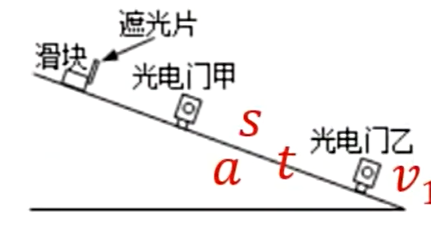
\includegraphics[width=0.35\linewidth]{image/1}
			\label{fig:1}
		\end{figure}
	\end{example}
	\vspace{1.3cm}
	\begin{example}
		一物体以初速度$v_0=20$m/s沿光滑斜面匀减速向上滑动,当上滑距离$x_0=30$m时,速度
		减为5m/s求运动的时间$t$的关系式是
	\end{example}
	\vspace{2cm}
	\begin{remark}
		上面的五大参数除了时间以外均为矢量,在规定正方向后,需要考虑正负
	\end{remark}
	\subsection{$A_{2}$平均速度和中间速度}
	\subsubsection{$A_{21}$平均速度}
	在这里,我们要注意到两个公式以及两个条件
	\begin{equation*}
		\bar{v}=\begin{cases}
			\frac{x}{t}\left( \text{所有条件均使用} \right)\\
			\frac{v_0+v_t}{2}\left( \text{仅限于匀变速直线运动} \right)\\
		\end{cases}
	\end{equation*}
	\subsubsection{$A_{22}$匀变速直线运动中的中间速度}
	中间时刻的瞬时速度:$v_{\frac{t}{2}}=\frac{v_0+v_t}{2} $
	
	中间位置瞬时速度:$v_{\frac{x}{2}}=\sqrt{\frac{{v_0}^2+{v_t}^2}{2}} $
	
	\begin{remark}
		$\text{比大小:当}a=0\text{时,}v_{\frac t2}=v_{\frac x2};\text{ 当}a\neq0\text{时,}v_{\frac t2}<v_{\frac x2}$
	\end{remark}
	\subsection{$A_{3}$直线运动中的陌生函数}
	套路:找准对应方程,化简,对比
	\begin{example}
		\begin{equation*}
			2s=t-t^{2}
		\end{equation*}
	\end{example}
	\vspace{1.3cm}
	\begin{example}
		\begin{equation*}
			5v=3+4t
		\end{equation*}
		\vspace{1.3cm}
	\end{example}
	\begin{example}
		\begin{equation*}
			-0.1v^{2}=2x-6
		\end{equation*}
	\end{example}
	\vspace{1.3cm}
	\subsection{$A_{4}$刹车陷阱}
	什么是刹车陷阱?刹车陷阱又称\textbf{停车陷阱,减速陷阱,掉头陷阱}
	\begin{example}
		一辆初速度为20m/s的汽车正在以大小为5m/$s^{2}$的加速度减速,求汽车在前5s内的位移。
	\end{example}
	\vspace{1.3cm}
	\begin{example}
			一辆初速度为20m/s的汽车正在以大小为-5m/$s^{2}$的加速度做变速运动,求汽车在前5s内的位移。
	\end{example}
	\vspace{1.3cm}
	\begin{remark}
		要注意停车时间!
	\end{remark}
	\section{$B$打点计时器全模型总结}
	\subsection{$B_{1}$打点计时器原理}
	\subsubsection{$B_{11}$电火花打点计时器}
	电火花打点计时器$\begin{cases}
		220V$\text{家用交流电}$\\
		$\text{电火花}+\text{墨粉盒}+\text{白纸}$\\
		$\text{电火花阻力小,频率稳定}$\\
	\end{cases}$
	\subsubsection{$B_{12}$电磁式打点计时器}
	电磁式打点计时器$\begin{cases}
		\text{低压学生交流电源}\\
		\text{电流}+\text{磁铁}+\text{振针}+\text{复写纸}\\
		\text{振针阻力大,频率不稳定}\\
	\end{cases}$
	\subsubsection{$B_{13}$配套仪器}
	配套仪器:\textbf{交流电源,开关,导线,纸带,刻度尺}
	\subsection{$B_{2}$打点计时器——计时原理}
	\subsubsection{$B_{21}$等时推论}
	等时推论:$\Delta s=aT^{2}=s_{2}-s_{1}=s_{3}-s_{2}=s_{4}-s_{3}=\cdots $
	(条件:\textbf{匀变速直线运动且时间间隔$T$相等})
	\begin{note}
		应用1:判断是否为匀变速直线运动
		
		\vspace{0.3cm}
		应用2:计算某一段的位移
	\end{note}
	\subsubsection{$B_{22}$打点周期$T$和计数点}
	为什么有些点不算数?
	
	起始段过于密集且不好测量,间隔取点可以有效减小测量误差
	
	\begin{remark}
		以下三句等价:
		
		1.每隔四个点取一个计数点
		
		2.每五个点中取一个计数点
		
		3.两个计数点之间有四个点未画出
	\end{remark}
	\vspace{-0.5cm}
	\subsection{$B_{3}$打点计时器——测量原理}
	\vspace{-0.5cm}
	\begin{figure}[H]
		\centering
		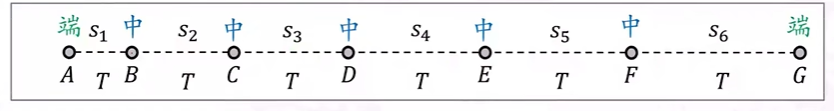
\includegraphics[width=0.8\linewidth]{image/2}
	\end{figure}
	\vspace{-0.5cm}
	\subsubsection{$B_{31}$测量速度}
	\begin{enumerate}
		\item $\text{平均速度}\bar{v}=\frac{s_{总}}{t_{总}}\quad v_{CE}=\frac{(s_{3}+s_{4})}{(2T)} $
		\item $\text{中点瞬时速度}v_{\text{中}}=\frac{(s_{\text{左}}+s_{\text{右}})}{t_{\text{总}}}\quad v_{B}=\frac{(s_{1}+s_{2})}{2T}\quad v_{E}=\frac{s_{4}+s_{5}}{2T}$
		\item $\text{端点瞬时速度}v_{\text{端}}=\frac{3s_{\text{邻}}-s_{\text{隔}}}{2T}\to v_{A}=\frac{3s_{1}-s_{2}}{2T}v_{G}=\frac{3s_{6}-s_{5}}{2T}$
	\end{enumerate}
	\subsubsection{$B_{32}$测量加速度}
	技巧:两端劈开,末减初,除以$nT^{2}$
	
	$\begin{aligned}&a=\frac{(s_{4}+s_{5}+s_{6})-(s_{1}+s_{2}+s_{3})}{9T^{2}}\\&a=\frac{(s_{4}+s_{5})-(s_{1}+s_{2})}{6T^{2}}\\&a=\frac{(s_{3}+s_{4})-(s_{1}+s_{2})}{4T^{2}}\\&a=\frac{s_{6}-s_{1}}{5T^{2}}
	\end{aligned}$
	\subsection{$B_4$其他类型打点计时器}
	\subsubsection{$B_{41}$滴水计时器}
	相同时间内滴下一滴墨水,以记录物体的位置信息(打点)
	\subsubsection{$B_{42}$频闪照相机}
	相同时间拍摄一张照片,以记录物体的位置信息(打点)
	\subsubsection{$B_{43}$通过点迹判断小车运动方向}
	打点计时器:先打出的点连接实物
\begin{figure}[H]
	\centering
	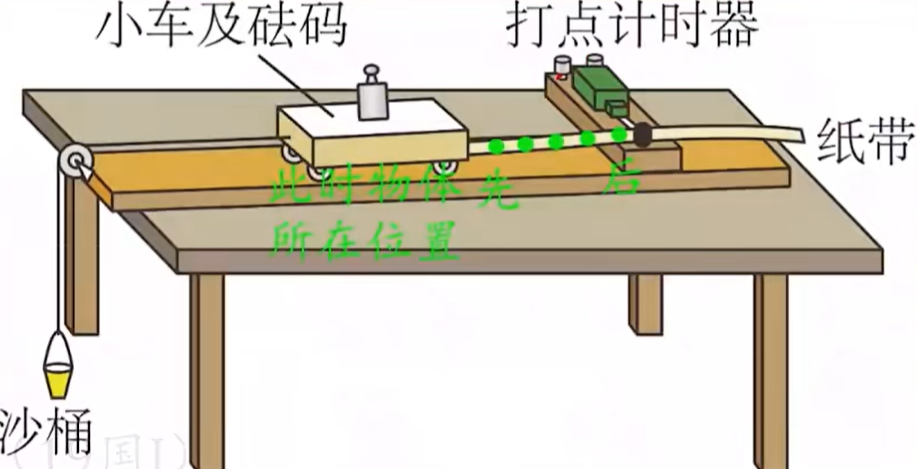
\includegraphics[width=0.5\linewidth]{image/4}
\end{figure}
	滴水计时器:后滴出的点靠近实物
	
	频闪照片:后闪出的点靠近小车
	\begin{figure}[H]
		\centering
		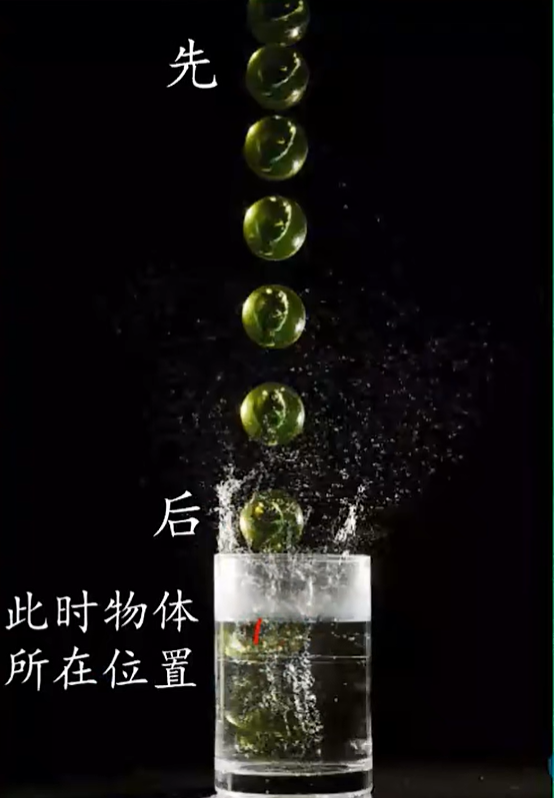
\includegraphics[width=0.2\linewidth]{image/5}
	\end{figure}
	\subsubsection{$B_{44}$曝光时间}
	定义:持续拍摄的时长($\Delta t)$ 
	
	底片:记录曝光时间内的轨迹($\Delta x$
	
	题型:计算平均速度$(\bar{v}=\frac{\Delta x}{\Delta t})$$\to $近似认为是瞬时速度$\upsilon$
	\section{$C$分段运动}
	\subsection{$C_{1}$等时分段运动}
	将其看作打点计时器的纸带即可
	
	\begin{example}
		已知$O,A,B,C$为同一直线上的四点,$AB$间的距离为$I_1,BC$间的距离为$I_2$,一物作自$O$点由静止出发,沿此直线做匀变速运动,依次经过 $A$、$B$、$C$ 三点,已知物体通过 $AB$ 段与$BC$段所用的时间相等。求$O$与$A$的距离。
	\end{example}
	\vspace{2cm}
	\subsection{$C_{2}$不等时分段运动}
	均速法
	
	两步走:
	\begin{enumerate}
		\item  画轴标时刻
		\item $\bar{v}\to v_\text{瞬}\to a\to\text{其他}$
	\end{enumerate}
	\vspace{2cm}
	\begin{example}
		一物体作匀加速直线运动,通过一段位移$\Delta x$  所用的时间为 $t_1$,紧接
		着通过下一段位移$\Delta x$  所用时间为$ t_2$,则物体运动的加速度为
	\end{example}
	\vspace{2cm}
	\section{$D$自由落体与竖直上抛}
	\subsection{$D_1$自由落体运动}
	\subsubsection{$D_{11}$自由落体运动的定义和公式}
	\begin{definition}
		初速度$v_0=0$,只受重力(不计空阻),加速度$a=g$的匀加速直线运动
	\end{definition}
	\begin{equation*}
		\begin{split}
			\text{缺}x\longrightarrow v_t=v_0+at\quad v=gt
			\\
			\text{缺}a\longrightarrow x=\frac{v_0+v_t}{2}t \quad h=\frac{v_t}{2}t
			\\
			\text{缺}v_t\longrightarrow x=v_0t+\frac{1}{2}at^2 \quad h=\frac{1}{2}gt^2
			\\
			\text{缺}t\longrightarrow 2ax=v_{t}^{2}-v_{0}^{2} \quad 2gh=v_{t}^{2}
		\end{split}
	\end{equation*}
	\subsubsection{$D_{12}$阻力对物体的影响}
	\subsubsection{$D_{13}$自由落体运动的三大题型}
	\textbf{题型一}:从顶端开始(利用好初始条件)
	\vspace{1.5cm}
	\begin{example}
		质量为$m$ 的物体从高为$h$ 处自由下落,开始的$\frac h3$用时为
		$t$,则( )
		
		 A. 物体接下来的$\frac{2h}{3}$所用的时间为 2$\iota$ 
		
		B. 物体落地所用的总时间为$\sqrt{3}t$
		
		C. 物体落地时的速度为$\sqrt{3}gt$
		
		D. 物体落地时的速度为 $3gt$
	\end{example}
	\vspace{1.8cm}
	\textbf{题型二}:有前看前,没前看第(前几秒,第几秒)
	\vspace{1.5cm}
	\begin{example}
		求自由落体运动第3秒内的位移h
	\end{example}
	
	\textbf{题型三}:非质点物体研究——专一
	\vspace{1.8cm}
	\subsection{$D_2$竖直上抛运动}
	\subsubsection{$D_{21}$三个重要量}
	
	最高点竖直方向速度:
	
	上升时间:
	
	最大高度:
	
	\vspace{2cm}
	
	\subsubsection{$D_{22}$对称性}
	同高等速率,上下等时间
	
	\begin{example}
		如图所示一跳水运动员从离水面10m高的平台上向上跃起,举双臂直体离开台面.此时其重心位于从手到脚全长的中点,跃起后重心升高0.45m 达到最高点,落水时身体竖直,手先入水(在此过程中运动员水平方向的运动忽略不
		计).从离开跳台到手触水面,他可用于完成空中动作的时间\_s(计算时,可以把运动
		员看作全部质量集中在重心的一个质点,g取$10m/s^2$,结果保留两位数字).
	\end{example}
	\begin{figure}[H]
		\centering
		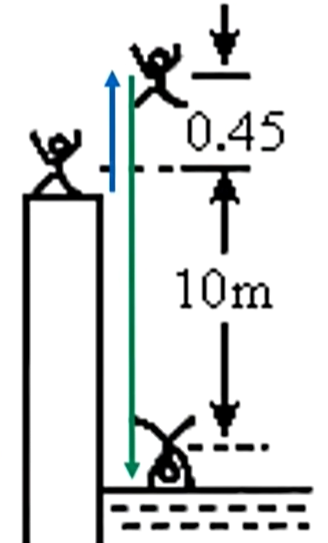
\includegraphics[width=0.2\linewidth]{image/7}
	\end{figure}
	\vspace{2cm}
	\section{$E$运动学图像归纳}
	\subsection{$E_1$位置时间(x-t)图}
	\begin{figure}[H]
		\centering
		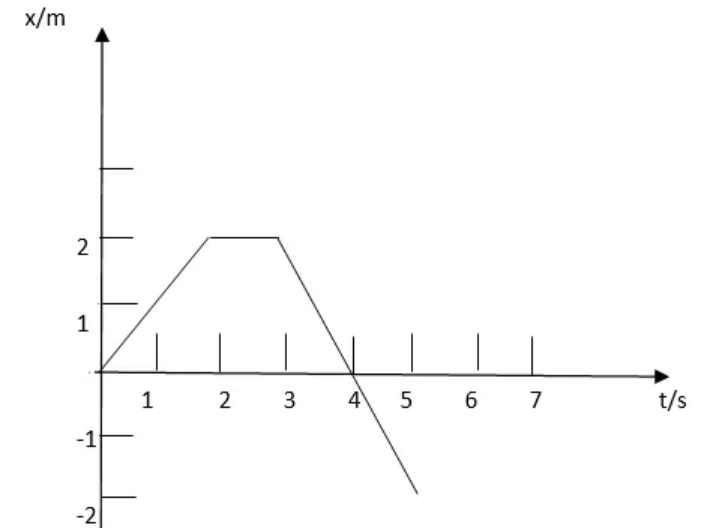
\includegraphics[width=0.3\linewidth]{image/8}
	\end{figure}
	\subsubsection{$E_{11}$理解横纵轴}
	$x:$相对于原点的位移
	
	$t:$时间
	
	$\Delta x$:位移
	
	$\Delta t$:时间间隔
	\subsubsection{$E_{12}$理解斜率}
	
	绝对值代表速度大小,正负代表方向
	\subsubsection{$E_{13}$面积}
	没意义
	\subsubsection{$E_{14}$图像交点}
	相遇
	\subsubsection{$E_{15}$图像零点}
	回到原点
	\subsubsection{$E_{16}$图像拐点}
	速度方向发生改变
	\subsection{$E_2$速度时间(v-t)图}
	\begin{figure}[H]
		\centering
		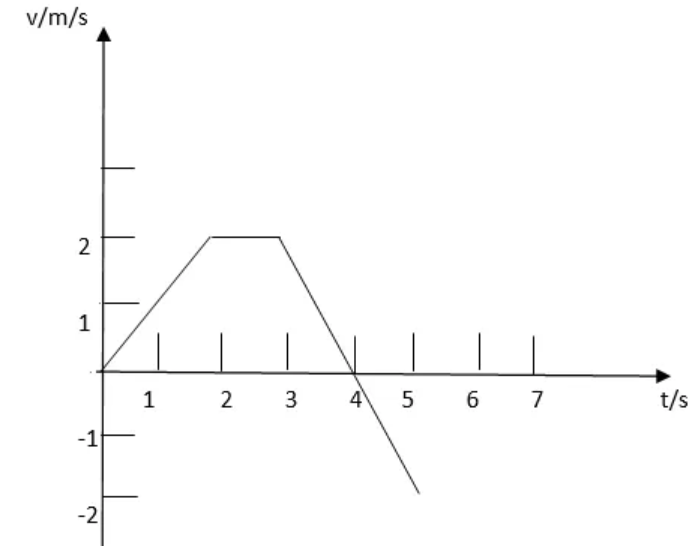
\includegraphics[width=0.3\linewidth]{image/9}
	\end{figure}
	
	\subsubsection{$E_{21}$理解横纵轴}
	$v:$瞬时速度
	
	$t:$时间
	
	$\Delta v$:速度变化量
	
	$\Delta t$:时间间隔
	\subsubsection{$E_{22}$理解斜率}
		绝对值代表加速度大小,正负代表方向
	\subsubsection{$E_{23}$面积}
	位移
	\subsubsection{$E_{24}$图像交点}
	共速
	\subsubsection{$E_{25}$图像零点}
	速度为零
	\subsubsection{$E_{26}$图像拐点}
	加速度方向改变
	\subsection{$E_3$加速度时间(a-t)图}
	\subsection{$E_4$其他类别图像}
	破题方法:五个运动学方程
	\subsubsection{$E_{41}$$\frac{x}{t}-t$图像}
	\vspace{2cm}
	\subsubsection{$E_{42}$$v^{2}-x$图像}
	\vspace{2cm}
	\subsubsection{$E_{43}$$x-t^{2}$图像}
	\vspace{2cm}
	\subsubsection{$E_{44}$$v-x$图像}
	\vspace{2cm}
	\section{$F$追击相遇模型}
	\subsection{$F_1$单物体多过程问题}
	\begin{figure}[H]
		\centering
		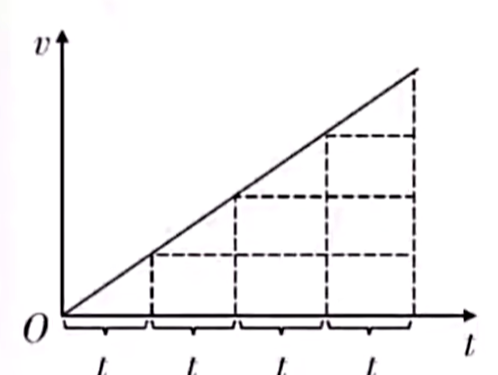
\includegraphics[width=0.35\linewidth]{image/10}
	\end{figure}
	\vspace{1cm}
	\begin{note}
		第$n$个时间$t$内的位移之比等于1:3: 5: 7......: (2n-1)
		
		前$n$个时间$t$内的位移之比等于1:4: 9: 16......: $n^2$
		
		第$n$个位移$x$内的时间之比等于1:$\sqrt2-1:\sqrt{3}-\sqrt2:\sqrt{4}-\sqrt3......:\sqrt{n}-\sqrt{n-1}$
		
		前$n$个位移$x$内的时间之比等于1:$\sqrt2:\sqrt{3}:\sqrt{4}......:\sqrt{n}$
	\end{note}
	\subsection{$F_2$多物体同时运动}
	\subsubsection{$F_{21}$共速点的运用}
	追击相遇问题中的\textbf{距离最值}
	\vspace{2.5cm}
	\subsubsection{$F_{22}$解追击相遇的基本套路}
	相遇情况分析:
	
	\vspace{3cm}
	利用共速点分析:
	\vspace{3cm}
	利用运动学方程求解:
	\vspace{3cm}
	\subsubsection{$F_{24}$两次相遇的特殊结论}
	$t_{1}+t_{2}=2t_{\text{共}}$
	\chapter{静力学模型}
	\section{$A$受力分析基础}
	\subsection{$A_{1}$刚绳弹力模型}
	常考的刚性光滑轻绳
	\subsubsection{$A_{11}$有结点刚性光滑轻绳}
	结点左右视为两条
	\subsubsection{$A_{12}$无结点刚性光滑轻绳}
	同条同力
	\begin{example}
		( 2024·浙江)如图所示,在同一竖直平面内,小球$A$、$B$上系有不可伸长的细线$a$、$b$、$c$和$d$,其中$a$ 的上端悬挂于竖直固定的支架上,$d$跨过左侧定滑轮、$c$跨过右侧定滑轮分别与相同配重$P$、Q相连周节左、右两侧定滑轮高度达到平衡。已知小球$A$、$B$和配重$P$、Q质量均为50$g$,细线$c$、$d$平行且与水平成$\theta=30°($ 不计摩擦),请做出$a$、$b$、$P$、$Q$的受力分析。
		\begin{figure}[H]
			\centering
			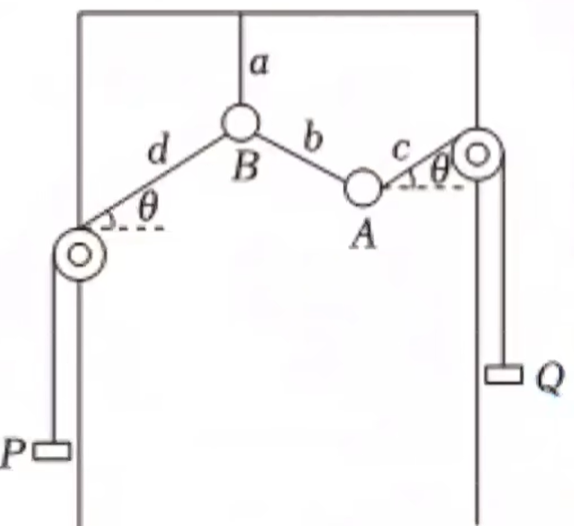
\includegraphics[width=0.4\linewidth]{image/11}
		\end{figure}
	\end{example}
	\subsection{$A_{2}$轻杆/硬杆弹力模型}
	\subsubsection{$A_{21}$死杆}
	$\begin{aligned}&\text{定义:固定不可动的杆(可直可弯)}\\&\text{特征:杆对其一端物体弹力满足“大小任意、方向任意”}\end{aligned}$
	\begin{figure}[H]
		\centering
		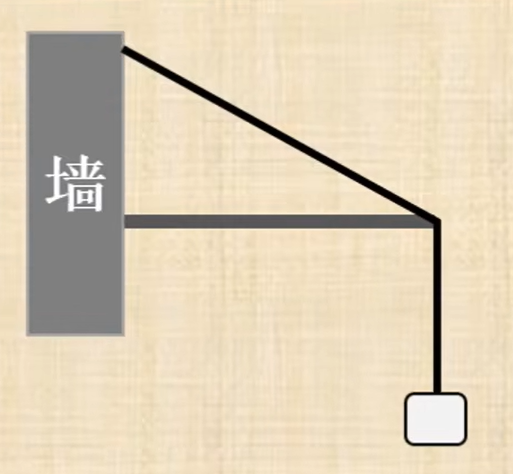
\includegraphics[width=0.2\linewidth]{image/15}
	\end{figure}
	
	\subsubsection{$A_{22}$活杆}
	$\text{一端铰接杆:杆对其一端的物体或受力点的弹力满足“大小任意、方向沿杆}$
	\begin{figure}[H]
		\centering
		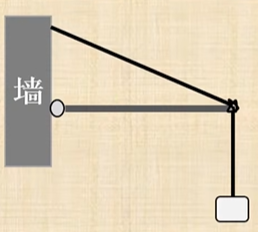
\includegraphics[width=0.2\linewidth]{image/16}
	\end{figure}
	
	$\text{两端自由杆:杆对其两端物体的弹力满足“方向沿杆、等大反向”}$
	\begin{figure}[H]
		\centering
		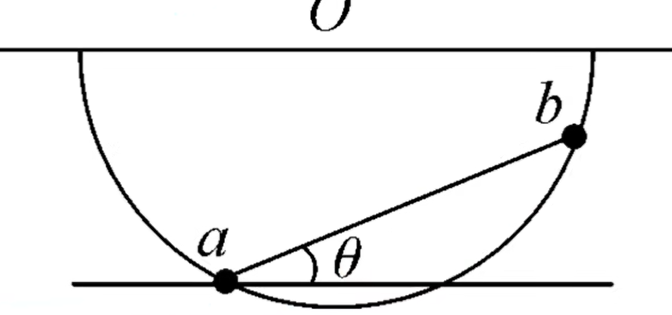
\includegraphics[width=0.3\linewidth]{image/21}
	\end{figure}
	
	\subsection{$A_{3}$接触类弹力模型}
	垂直于接触面,指向受力物体
	\subsubsection{$A_{23}$目标杆}
	杆作为受力分析的目标来出现,需要考虑重力
	\begin{example}
		如图所示,一轻质晒衣架静置于水平地面上,水平横杆与四根相同的斜杆垂直,两
		斜杆夹角$\theta=60°$。一重为$G$的物体悬挂在横杆中点,请对任一斜杆做受力分析。
		\begin{figure}[H]
			\centering
			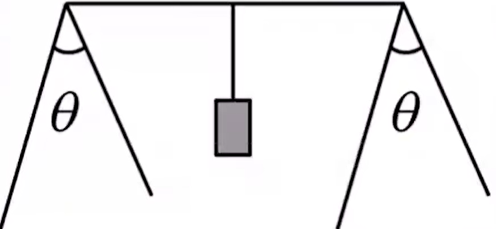
\includegraphics[width=0.4\linewidth]{image/12}
		\end{figure}
	\end{example}
	\vspace{2cm}
	\subsection{$A_{4}$初见弹簧}
	\subsubsection{$A_{41}$胡克定律}
	$\begin{aligned}\\F_{\text{ 弹}}=k\cdot\Delta x=\begin{cases}\text{弹簧弹力F}\text{弹怎么看?一一}F_{\text{弹 }}=F_\text{左}=F_\text{右}\\\text{劲度系数k的几何意义?——}F-L\text{图像或}F-\Delta x\text{图像的斜率}\\\text{形变量$\Delta $x怎么算?——看到弹簧先标原长,总 长度之差}\end{cases}\end{aligned}$
	\subsubsection{$A_{42}$弹簧并联}
	\vspace{2cm}
	\subsubsection{$A_{43}$弹簧串联}
	\vspace{2cm}
	\subsection{$A_{5}$三种摩檫力}
	\subsubsection{$A_{51}$静摩檫力}
	被动力:静摩檫力是块砖,哪里需要那里搬
	\vspace{2cm}
	
	\begin{remark}
		一般认为最大静摩檫力和滑动摩檫力相等
	\end{remark}
	除此之外,还需要记住一个模型:
	\vspace{2.5cm}
	\subsubsection{$A_{52}$滑动和滚动摩檫力  }
	“3+1”方程:$f=\mu F_N,F_N=N,N=?,f=?$
	
	条件:接触、挤压、粗糙、相对运动
	\vspace{3cm}
	
	摩檫力方向判断:同向运动,快反慢同,其他情况,$fv$相反
	\vspace{3cm}
	
	不管是动摩擦力还是静摩擦力:
	
	摩擦力既能使物体加速也能减速;
	
	摩擦力既能促进物体运动也能阻碍物体运动;
	
	摩擦力既能对物体做正功也能做负功还能不做功:
	
	摩擦力既能与运动方向相同,也能与运动方向相反,还能与运动方向垂直。
	\subsection{$A_{6}$力的合成与分解}
	\subsubsection{$A_{61}$力的合成}
	\vspace{4cm}
	\subsubsection{$A_{62}$力的分解}
	$\begin{aligned}&\text{当合力的大小和方向一定时,若:}\\&1.\text{已知两个分力的方向,求两个分力的大小}\\&2.\text{已知一个分力的大小和方向,求另一个分力的大小和方向}\\&3.\text{已知两个分力的大小,求两个分力的方向};\\&4.\text{已知一个分力的大小和另一个分力的方向,求这两个分力的大小和方向}\end{aligned}$
	\vspace{3cm}
	\subsection{$A_{7}$受力分析}
	口诀:一重二弹三摩擦,四电五磁六其它
	
	\begin{remark}
		
		重:要明确研究对象
		
		弹:找绳找杆找弹簧,绕物一圈找接触
		
		摩擦:先接触再摩擦
	\end{remark}
	\begin{example}
		\begin{figure}[H]
			\centering
			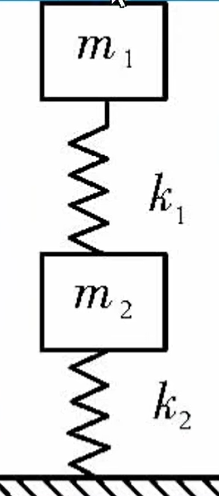
\includegraphics[width=0.1\linewidth]{image/13}
		\end{figure}
	\end{example}
	\begin{example}
		\begin{figure}[H]
			\centering
			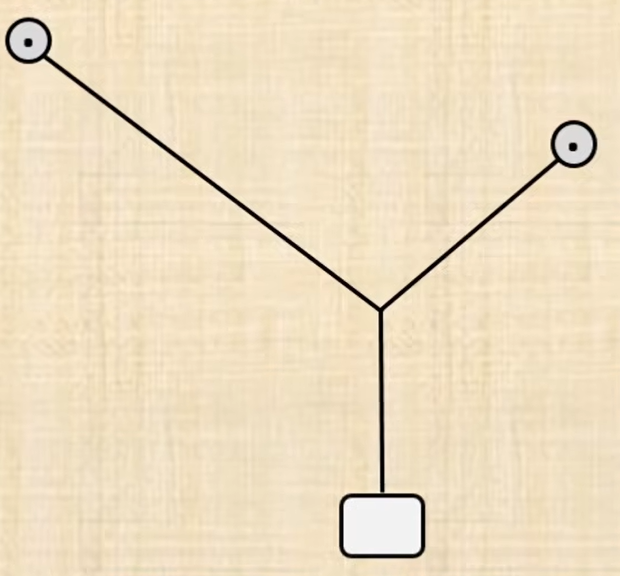
\includegraphics[width=0.2\linewidth]{image/14}
		\end{figure}
	\end{example}
	\begin{example}
		\begin{figure}[H]
			\centering
			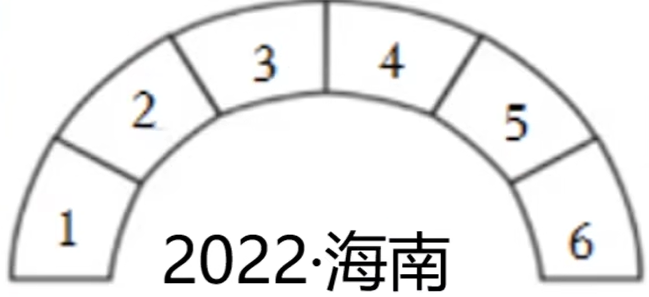
\includegraphics[width=0.24\linewidth]{image/17}
		\end{figure}
	\end{example}
	\begin{example}
		\begin{figure}[H]
			\centering
			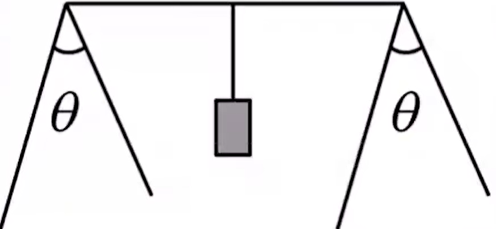
\includegraphics[width=0.4\linewidth]{image/12}
		\end{figure}
	\end{example}
	\begin{example}
		\begin{figure}[H]
			\centering
			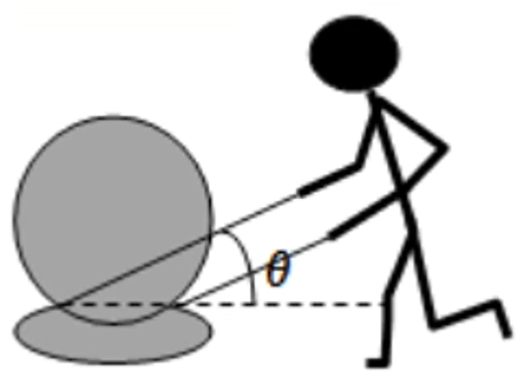
\includegraphics[width=0.3\linewidth]{image/18}
		\end{figure}
	\end{example}
	\begin{example}
		\begin{figure}[H]
			\centering
			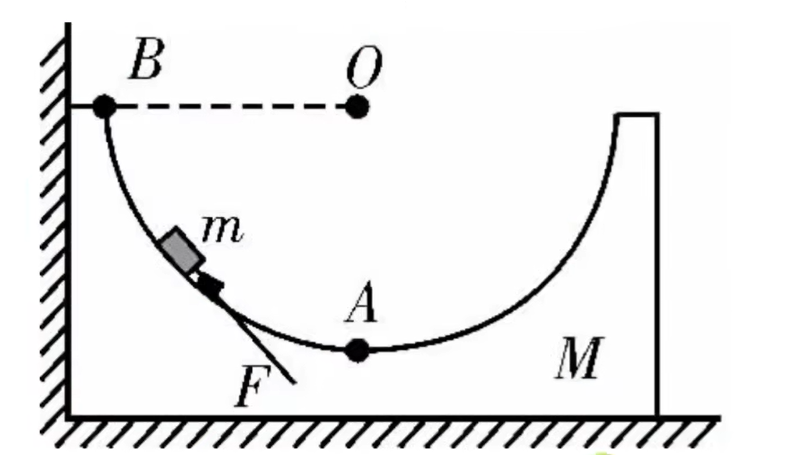
\includegraphics[width=0.3\linewidth]{image/19}
		\end{figure}
	\end{example}
	\begin{example}
		\begin{figure}[H]
			\centering
			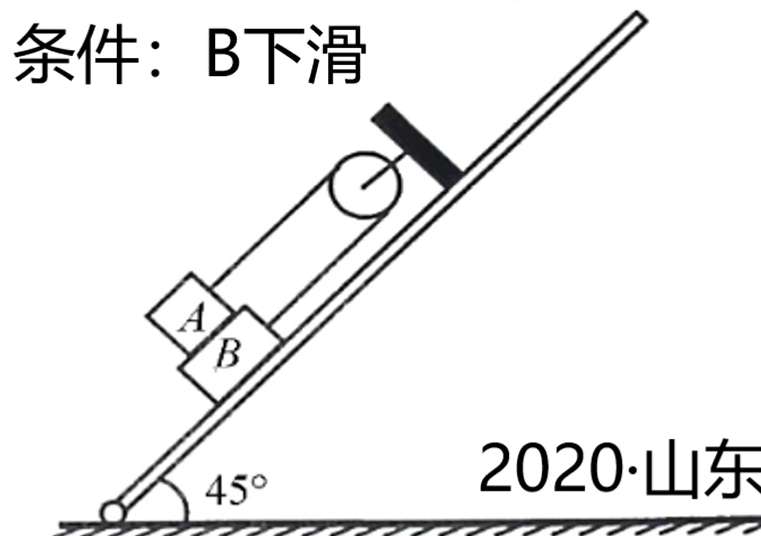
\includegraphics[width=0.25\linewidth]{image/20}
		\end{figure}
	\end{example}
	\section{$B$静力学模型}
	\subsection{$B_{1}$力的分类和三力交汇}
	\subsubsection{$B_{11}$力的三分类}
	
	恒力:方向不变,大小不变
	
	定力:方向不变,大小变化
	
	变力:方向变化,大小随意
	 
	
	都是恒力——静态平衡
	
	有定有变——
$	\text{动态平衡}\begin{cases}
		\text{恒定变}\\
		\text{恒两变}\begin{cases}
			\text{相似三角形}\\
			Y\text{型平衡}\\
			\text{定角型}\\
			\text{非定角型}\\
		\end{cases}\\
	\end{cases}$
	\subsubsection{$B_{13}$三力交汇原理}
	$\begin{aligned}&1.\text{若物体处于三力平衡状态,则}\text{三力延长线必交于一点;}\\&\text{2.高中阶段只研究共点力平衡;}\\&\text{3.高中阶段力可以进行平移。}\end{aligned}$
	\begin{example}
		\begin{figure}[H]
			\centering
			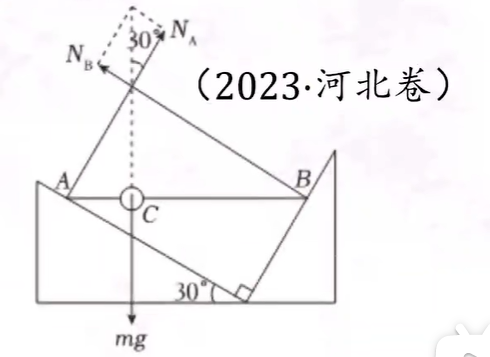
\includegraphics[width=0.3\linewidth]{image/22}
		\end{figure}
	\end{example}
	\subsection{$B_{2}$三力静态平衡}
	方法很多,有正交分解法这些,这里只推荐一个方法,外正弦定理法
	\begin{figure}[H]
		\centering
		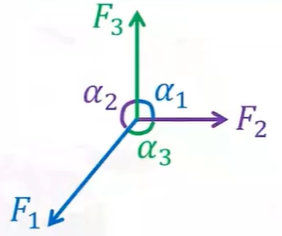
\includegraphics[width=0.3\linewidth]{image/23}
	\end{figure}
	我们有
	\begin{equation*}
		\frac{F_1}{\mathrm{sin}\alpha_1}=\frac{F_2}{\mathrm{sin}\alpha_2}=\frac{F_3}{\mathrm{sin}\alpha_3}
	\end{equation*}
	
	大题怎么写?由平衡关系可知
	\subsection{$B_{3}$三力动态平衡}
	\subsubsection{$B_{31}$三力动态平衡-恒定变}
	套路:恒力反向、定力平移(虚线延长)、变力旋转(平?陡?)
	
	\begin{example}
		\begin{figure}[H]
			\centering
			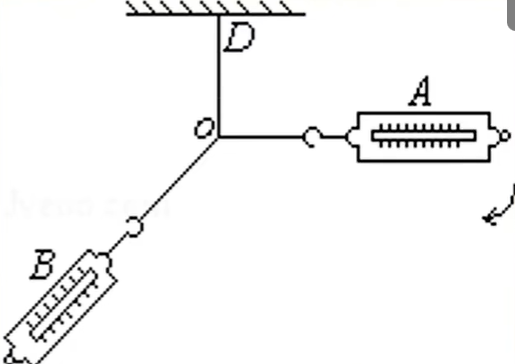
\includegraphics[width=0.4\linewidth]{image/24}
		\end{figure}
		
		$\begin{aligned}&\text{如图所示,用两个弹簧秤A和B,互成角度地拉}\text{橡皮条,使结点0达到图中所示位置,在保持O点位置}\\&\text{和B弹簧秤拉力方向不变的情况下,将弹簧秤A缓慢地}\text{沿顺时针方向转动,那么在此时程中,A与B的示数将}\\&\text{分别()}\\&\text{A.变大;变小}\\&\text{B.变小;变小}\\&\text{C.先变小再变大;变小}\\&\text{D.先变大再变小;变大}\end{aligned}$
	\end{example}
	\begin{conclusion}
		定变垂直最小
	\end{conclusion}
	
	\subsubsection{$B_{32}$三力动态平衡-恒两变}
	
	\textbf{类型一:相似三角形}
	
	适用情况:一恒两变,一眼有三角形
	
	做题套路:力的矢量三角形相似于几何三角形
	\begin{example}
\begin{figure}[H]
	\centering
	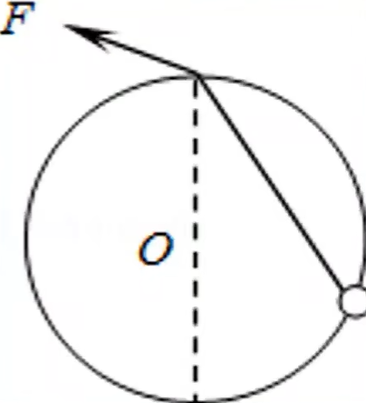
\includegraphics[width=0.14\linewidth]{image/26}
\end{figure}
		如图所示,固定在竖直平面内的光滑圆环的最高点有一个光滑的小孔.质量为m 的小球套在圆环上。一根细线的下端系着小球,上端穿过小孔用手拉住。现拉动细线,使小球沿圆环缓慢上移。手对线的拉力为F,轨道对小球的弹力为N,则
		
		A. $F$不变,$N$增大
		
		B. $F$不变,$N$ 减小
		
		C .$F$减小,$N$不变 
		
		D.$F$增大,$N$减小
	\end{example}
	\vspace{1cm}
	\textbf{类型二、Y型平衡}
	\begin{figure}[H]
		\centering
		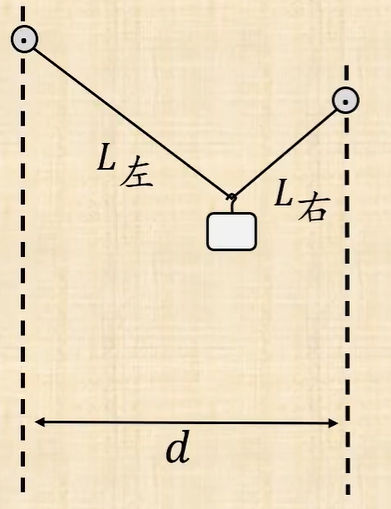
\includegraphics[width=0.3\linewidth]{image/27}
	\end{figure}
	
	考点一、角等力等
	\vspace{2cm}
	
	考点二、角大力大
	
	$\alpha$和$F$的关系?
	\vspace{2cm}
	
	$\begin{aligned}
		&\text{钉子上下移动(}d\text{不变},\alpha \text{不变}\\
		&\text{钉子左右移动(}d\text{变},\alpha \text{变)}\\
		&\text{绳子总长变短}\\
		&\text{绳子总长变长}\\
	\end{aligned}$
	\vspace{1cm}
	
	\textbf{类型三:定角型}
	
	套路:外正弦定理(拉米定理)
	\begin{example}
		\begin{figure}[H]
			\centering
			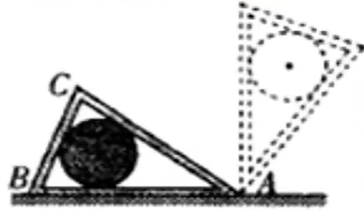
\includegraphics[width=0.4\linewidth]{image/28}
		\end{figure}
		如图所示,水平面上等腰三角形均匀框架顶角$\angle$BAC=
		$30^{\circ}$,一均匀圆球放在框架内,球与框架BC、AC两边接触但无挤压,现使框架以顶点
		A为转轴在竖直平面内顺时针方向从AB边水平缓慢转至AB边竖直,则在转动过程中
		
		A. 球对AB边的压力先增大后减小
		
		B. 球对BC边的压力先增大后减小
		
		C. 球对AC边的压力先增大后减小
		
		D. 球的重力势能一直增大
	\end{example}
	
	\textbf{类型四:非定角型}
	
	套路:恒力反向,随便一个力平移,两个变力一起旋转
	
	\begin{example}
		$\text{已知}F_1\mathrm{,}F_2\text{逆时针旋转,求}F_1\mathrm{,}F_2\text{大小变化情况。}$
	\end{example}
	\vspace{3cm}
	\begin{conclusion}
		套路总结
		
		$\begin{aligned}&\text{【恒定变】-恒反、定平、变旋}\\&\text{【恒两变/相似三角形】-恒反、随平}\\&\text{【恒两变/非定角型】-恒反、随平、变旋}\end{aligned}$
	\end{conclusion}
	\section{$C$系统}
	
	$\text{内力:施力物体和受力物体都在系统内}$ 
	
	$\text{外力:施力物体和受力物体有一个在系统外}$
	\subsection{$C_{1}$整体法}
$	\text{整体法}\begin{cases}\text{when? 求系统外力的时候}\\\text{how? 只分析外力}\end{cases}$
	\subsection{$C_{2}$隔离法}
	$\text{隔离法}\begin{cases}
		\mathrm{when}? \text{求系统内力的时候}\\
		\mathrm{how}? \text{分析所有的力}\\
	\end{cases}$
	
	\begin{example}
		\begin{figure}[H]
			\centering
			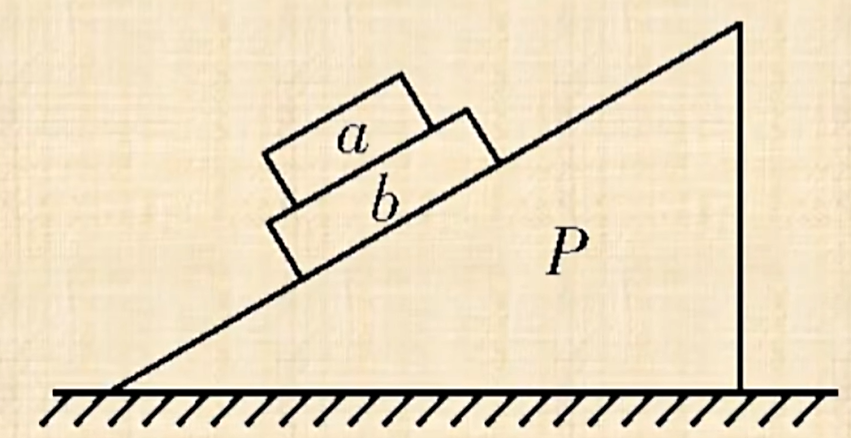
\includegraphics[width=0.3\linewidth]{image/29}
		\end{figure}
	\end{example}
	\vspace{3cm}
	\section{$D$多物体平衡}
	\subsection{$D_{1}$正交分解}
	$\text{正交方向选择}\left\{ \begin{array}{c}
		\text{有斜面}:\text{沿斜面和垂直于斜面分解}\\
		\text{有绳杆}:\text{沿绳}/\text{杆和垂直于绳}/\text{杆方向分解}\\
		\text{有运动}:\text{沿运动方向和垂直于运动方向}\\
		\text{哈也没有}:\text{沿水平和竖直方向分解}\\
	\end{array} \right. $
	\subsection{$D_{2}$全反力和全反角}
	
	条件:滑动摩檫力
	
	定义:全反力$R$,全反角$\alpha$
	\begin{conclusion}
		恰好开始运动-恰好构成闭合的矢量三角形 
		
		加速状态-构成矢量三角形,且$F$穿透全反力
		
		自锁-构成不了矢量三角形(平行恰好)
	\end{conclusion}
	\vspace{6cm}
	\chapter{牛顿定律模型}
	\section{$A$牛顿定律三大基础题型}
	\subsection{$A_1$状态写牛二}
	$a\left\{ \begin{array}{c}
		\text{运动状态}\begin{cases}
			\text{匀速、匀加、匀减、匀圆}\\
			\text{最大速度}/\text{最小速度}\rightarrow a=0\\
		\end{cases}\\
		\text{临界状态} \text{绳子刚好被拉断}/\text{桌子刚好离地}/\text{车刚好被推动}\\
	\end{array} \right. $
	
$	F_{\text{合}}=ma\left\{ \begin{array}{c}
		\text{注意矢量方向}\\
		\text{达朗贝尔原理}—\text{反向添加}ma\text{当作平衡}\\
	\end{array} \right. $
	\vspace{2cm}
	\subsection{$A_2$牛二的系统应用一:牛顿质点系方程}
	应用场景:A物体的受力$\leftrightarrow$B物体的运动状态
	
	基本套路:
	
	step1: 只分析外力
	
	step2: 反向添加$ma$视为惯性力
	
	step3:写平衡方程
	
	\begin{remark}
		力和加速度要分别列在等式的两边
	\end{remark}
	\begin{example}
		$M\text{静止,}m\text{加速下滑,已知}m\mathrm{,}M\mathrm{,}\theta\mathrm{,}a\text{,求地面对}M\text{的支持力}N\text{和摩擦力}f$
		\begin{figure}[H]
			\centering
			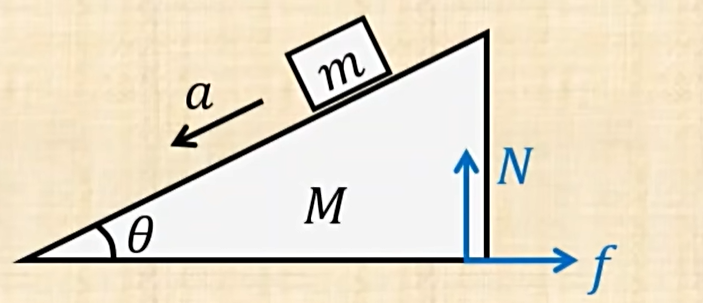
\includegraphics[width=0.3\linewidth]{image/30}
		\end{figure}
		
	\end{example}
	\subsection{$A_3$加速度图像}
	\subsubsection{$A_{31}$$a-t$图$(F-t)$图}
$	\begin{aligned}&\text{做题套路:}F-t\text{图像}\to F_\text{合}-t\text{图像}\to a-t\text{ 图像}\to v-t\text{图像}\\&\text{图像面积:}a\cdot t=\Delta v=v_\text{末}-v_\text{初}\end{aligned}$
    \subsubsection{$A_{32}$$a-x$图}
    $\text{图像面积:}a\cdot x=\frac12(v_\text{末}^2-v_\text{初}^2)\quad“a-x\text{图像的面积代表的含义是速方差的一}$
    \subsubsection{$A_{33}$典型的$a-t$图}
    \vspace{3cm}
    \section{$B$斜面问题和等时三角形}
    \subsection{$B_{1}$物体在斜面上的运动分析}
    \subsubsection{$B_{11}$受力分析和加速度}
    \vspace{3cm}
    \subsubsection{$B_{12}$$\mu$与$tan$关系}
    $\mu\text{与tan关系}\left\{\begin{array}{ll}\text{静止、减速下滑}&\mu>\tan\theta\\\text{恰好静止、匀速下滑}&\mu=\tan\theta\\\text{加速下滑}&\mu<\tan\theta\end{array}\right.$
    \subsubsection{$B_{13}$斜面上的全反力(难)}
    \vspace{2cm}
    \subsection{$B_{2}$等效重力场}
     \subsubsection{$B_{21}$等效质量}
     相对静止的多个物体可以看成整体
     \subsubsection{$B_{22}$等效重力加速度}
     外力型等效
     
     $\begin{aligned}&\overrightarrow{G'}=\overrightarrow{mg}+\overrightarrow{F}\\&\overrightarrow{g'}=\frac{mg+F}{m}=\overrightarrow{g}+\frac{\overrightarrow{F}}{m}\end{aligned}$
     
     加速型等效
     
     $\overrightarrow{G^{\prime}}=\overrightarrow{mg}+\overrightarrow{F_{\text{惯}}}$
     
     $g^{\prime}=g+a_{\text{反}}$
     \subsection{$B_{3}$等时三角形/等时圆}
     $\text{【场景】初速度为0的物体在光滑斜面上的运动时间}$
     
     $\text{【套路】一端找竖直,一端找垂直}$
     \vspace{3cm}
     \section{$C$连接体问题全解}
     \subsection{$C_{1}$质量分配原理}
     
     质量分配原理:外力按照质量进行分配
     
     类型一:水平连接,一个外力
     \begin{figure}[H]
     	\centering
     	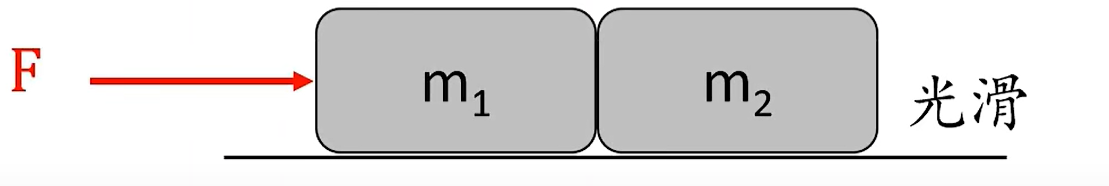
\includegraphics[width=0.4\linewidth]{image/31}
     \end{figure}
     
     类型二:水平连接,两个外力
\begin{figure}[H]
	\centering
	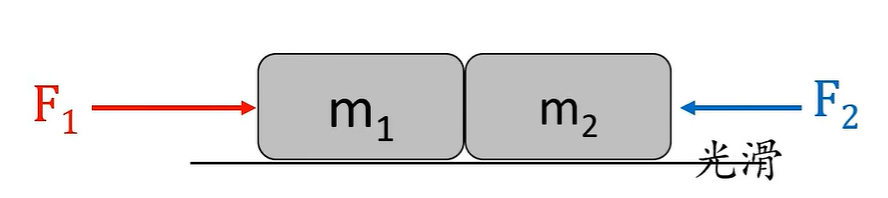
\includegraphics[width=0.4\linewidth]{image/33}
\end{figure}
     \begin{remark}
     	物体此时分配的外力之和则为物体此时受到的合外力
     \end{remark}
     \subsubsection{$C_{12}$内力法则}
    $ \text{内力法则}\left\{ \begin{array}{c}
     	\text{内力等于被动体分配的外力之和}\\
     	\text{忽略与质量成正比的外力(重力、下滑力、等$ \mu$摩擦外力)}\\
     	\text{同向相加,反向相减(仅计算内力)}\\
     \end{array} \right. $
\begin{figure}[H]
	\centering
	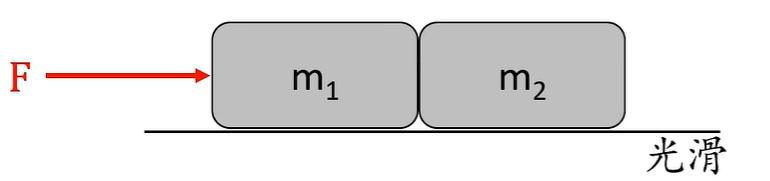
\includegraphics[width=0.4\linewidth]{image/36}
\end{figure}
     \begin{figure}[H]
     	\centering
     	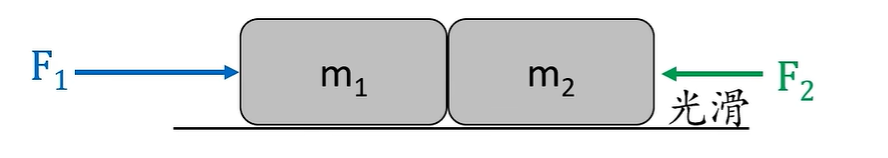
\includegraphics[width=0.4\linewidth]{image/35}
     \end{figure}
    
    类型三:水平连接,等$ \mu$摩擦外力
    \begin{figure}[H]
    	\centering
    	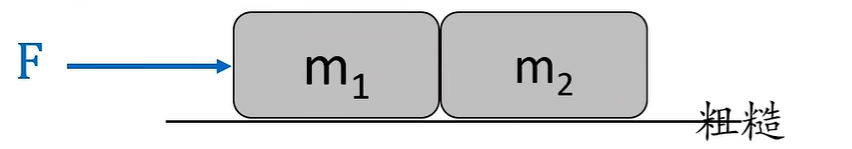
\includegraphics[width=0.4\linewidth]{image/37}
    \end{figure}
    \begin{remark}
    	作用在同一个物体上的力才可以合成
    \end{remark}
    
    类型四:水平连接,不等$ \mu$摩擦外力
    
    \begin{figure}[H]
    	\centering
    	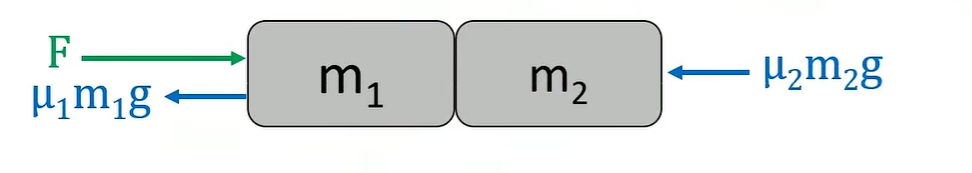
\includegraphics[width=0.4\linewidth]{image/38}
    \end{figure}
    
    类型五:叠加连接体
    \begin{figure}[H]
    	\centering
    	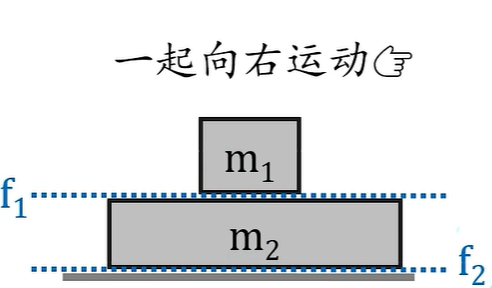
\includegraphics[width=0.4\linewidth]{image/39}
    \end{figure}
    \subsubsection{$C_{13}$用质量分配判断相对滑动}
    \begin{figure}[H]
    	\centering
    	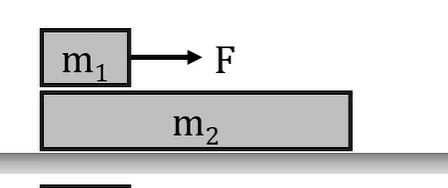
\includegraphics[width=0.4\linewidth]{image/40}
    \end{figure}
    \vspace{3cm}
    \begin{remark}
    	相对滑动的条件:将计算内力和实际内力比较
    \end{remark}
      \subsection{$C_{2}$牛二的系统应用二:轻绳滑轮连接体}
      
      方法:利用轻绳的五个相等,状态写牛二
      
      $\begin{aligned}&\text{同一条绳子拉力}T\text{相等}\\&\text{绳两端沿绳方向位移}x\text{相等}\\&\text{绳两端沿绳方向速度}v\text{相等}\\&\text{绳两端沿绳方向加速度}a\text{相等}\end{aligned}$
      \begin{figure}[H]
      	\centering
      	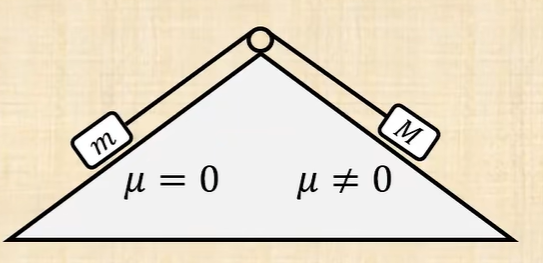
\includegraphics[width=0.3\linewidth]{image/41}
      \end{figure}
       \subsection{$C_{3}$不共线连接体}
       当物体运动和力不共线时
       \vspace{3cm}
       \begin{example}
       	长方体$A$、$B$置于粗糙水平地面上,$A$和$B$质量相同与地面的动摩擦因数也相同。左图中、对$A$施加水平向右、大小为F的推力时,$A、B$间的弹力大小为$F_1$;右图中,对$A$ 施加与水平方向成60°斜向下、大小为$2F$的推力时,$A$、$B$ $\text{间的弹力大小为}F_2$。两图中的$A$、$B$均做匀加速直线运动,则( ) 
       	
       	$\mathrm{A.}F_{1}<F<F_{2}$
       	
       	$\mathrm{B.}F_{1}<F_{2}<F$
       	
       $	\mathrm{C.}F_{1}=F_{2}<F$
       	
       	$\mathrm{D.}F_{2}<F_{1}<F$
       	\begin{figure}[H]
       		\centering
       		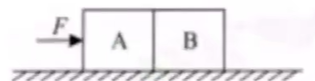
\includegraphics[width=0.3\linewidth]{image/42}
       		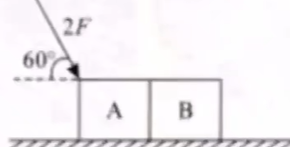
\includegraphics[width=0.3\linewidth]{image/43}
       	\end{figure}
       	
       \end{example}
       \subsection{$C_{4}$不共线连接体:内力加速度不共线}
       \vspace{3cm}
       \section{$D$弹力突变与瞬时加速度问题}
       \subsection{$D_{1}$弹簧的突变问题}
       \subsubsection{$D_{11}$弹簧弹力的存在条件}
       弹簧弹力的存在条件:弹簧发生形变且两端存在约束
       
       高中阶段研究的弹簧只是力传递的媒介
       \subsubsection{$D_{12}$剪断弹簧的解释}
       $\text{剪断弹簧}\begin{cases}
       	\text{力的角度解释:剪断后与施}/\text{受力物体分开}\rightarrow \text{弹簧弹力突变为}0\\
       	\text{功的角度解释:弹簧具有弹性势能}\rightarrow \text{剪断后弹性势能不能凭空消失}\\
       \end{cases}$
       \subsubsection{$D_{13}$不剪断弹簧}
       不剪短弹簧:弹簧弹力瞬间不变
       
       \subsection{$D_{2}$轻绳的突变问题}
       \subsubsection{$D_{21}$刚绳弹力的存在条件}
       刚绳弹力的存在条件:绷直且两端存在约束
       
       高中阶段研究的弹簧只是力传递的媒介
       \subsubsection{$D_{22}$剪断刚绳}
    弹力突变为零
       \subsubsection{$D_{23}$不剪断刚绳}
       不剪断:$\text{绳两端都可以运动且保持相对静止(动动类型)}$
       
       绳子两端加速度相等
       
         不剪断:$\text{绳一端固定另一端做圆周运动(动定类型)}$
         
         沿着绳子方向合外力为0
         \subsection{$D_{3}$接触类弹力突变问题}
         存在条件:接触。挤压(缺一个弹力变成0)
         
         \begin{example}
         	\begin{figure}[H]
         		\centering
         		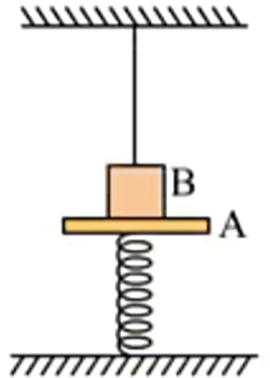
\includegraphics[width=0.2\linewidth]{image/44}
         	\end{figure}
         	$\begin{aligned}&\text{如图,质量为3kg的物体A静止在竖直的}\text{轻弹簧上,质量为2kg的物体B用细线悬挂,A与B}\\&\text{间相互接触但无压力,重力加速度}g=10\mathrm{m/s}^2。\text{某时刻将细线剪断,则细线剪断瞬间}\\&\text{A. 物体A的加速为零。}\\&\text{B. 弹簧弹力大小为30N}\\&\text{C. 物体B的加速度大小为4m/s}^2\\&\text{D. 物体B对物体A的压力大小为12N}\end{aligned}$
         	
         	
         \end{example}
         \subsection{$D_{4}$摩檫力突变问题}
        $ \text{存在条件:接触、挤压、粗糙、相对运动/相对运动趋势}$
        \section{$E$超失重与弹簧振子}
        \subsection{$E_{1}$超重失重}
        $\text{超重:加速度}a\text{向上 地面支持力}N>mg\\\text{失重:加速度}a\text{向下 地面支持力}N<mg\\\text{完全失重:加速度}a=g\text{向下 地面支持力}N=0$
        \subsection{$E_{2}$弹簧单振子(三段式、五段式)}
        \vspace{3cm}
        \subsection{$E_{3}$弹簧双振子的分离特性}
        何时分离?初速度不同肯定分离,初速度相同时两物体中间弹力为零时候分离
        \begin{example}
        	初始情况下,$m_1$、$m_2$静止,现恒力F作 用于$m_1$上,请求出二者分 离时弹簧的形变量?
        \end{example}
        \vspace{2cm}
        \begin{example}
        	$\text{初始情况下},m_1\text{、}m_2\text{静止},m_2\text{和弹簧栓接},\text{现给}m_1\text{和}m_2\text{共同向上的初速度}v_0,\text{若二者最终分离},\text{请求出分离时弹簧的形变量。}
        	$
        \end{example}
        \vspace{2cm}
        \section{$F$板块运动五步法}
        \subsection{$F_{1}$板块运动位移关系}
        单过程运动:
        \vspace{3cm}
        \subsection{$F_{2}$板块运动五步法}
        $\begin{aligned}&\text{Step1:判断}f\text{方向和大小}\\&\text{Step2:状态写牛二}\\&\text{Step3: 匀变画图像}\\&\text{Step4:对着图像列方程}\\&\text{Step5:通过面积求}\Delta s\text{、}s_\text{板、}s_\text{物}\end{aligned}$
        \begin{example}
        	质量为0.45kg的木块静止在光滑水平面上,一质量为0.05kg的子弹以200m/s 的水平速度击中木块,并留在其中,整个木块沿子弹原方向运动,若子弹在木块中运动时受到的平均阻力为$f$ =$4.5\times10^{3}$N,则:(1)木块最终速度的大小是(2)则子弹射入木块的深度为
        \end{example}
        \vspace{3cm}
        \section{$G$空气阻力下的直线运动}
         \subsection{$G_{1}$通性解法}
         核心方法:求解加速度$a$
         
         $\text{阻力类型}\begin{cases}
         	\text{阻力为定值}\rightarrow \text{匀变速直线运动}\rightarrow \text{匀变五大方程分析参数}\\
         	\text{阻力和速率成正相关}\rightarrow \text{变加速直线运动}\rightarrow \text{特殊位置}/\text{状态}\\
         	\text{阻力和体积}/\text{半径成正相关}\rightarrow \text{匀变速直线运动}\rightarrow \text{匀变五大方程分析参数}\\
         \end{cases}$
         \vspace{3cm}
         \section{$H$四类传送带问题}
         \subsection{$H_{1}$水平同向(共速趋势)}
         
         共速讨论:$ \boldsymbol{L}\text{比较}\boldsymbol{S}_{\text{共}}\left\{ \begin{array}{c}
         	\boldsymbol{L}>\boldsymbol{S}_{\text{共}}\,\,\text{先加速后匀速到共速}\\
         	\boldsymbol{L}=\boldsymbol{S}_{\text{共}}\,\,\text{加速至恰好共速}\\
         	\boldsymbol{L}<\boldsymbol{S}_{\text{共}}\,\,\text{加速未共速}\\
         \end{array} \right. $
         
          \subsection{$H_{2}$水平反向(共速趋势)}
         
         减速讨论:$\boldsymbol{L}\text{比较}\boldsymbol{S}_{\text{共}}\left\{ \begin{array}{c}
         	\boldsymbol{L}>\boldsymbol{S}_{\text{共}}\,\,\text{浪子回头}\\
         	\boldsymbol{L}=\boldsymbol{S}_{\text{共}}\,\,\text{悬崖勒马}\\
         	\boldsymbol{L}<\boldsymbol{S}_{\text{共}}\,\,\text{掉下去了}\\
         \end{array} \right. $
         
         \subsection{$H_{3}$倾斜向上传送带(先加再匀)}
         前提条件:μ一定大于tanθ
         
         $a$=
         
         \subsection{$H_{4}$倾斜向下传送带(先加再匀)}
         $\text{若μ<tan}\theta:\text{ 一加再加}$
         
         $a_1$=
         
         $a_2$=
         
         $\text{若μ>tan}\theta:\text{ 先加后匀}$
         
          $a_1$=
         
         $a_2$=
         \chapter{曲线运动}
         \section{$A$曲线运动基本概念}
        $\text{曲线运动的速度}\begin{cases}
        	\text{曲线运动的速度方向是轨迹的切线方向}\\
        	\text{由于速度方向会变,所以曲线运动是变速运动}\\
        	v\text{和}a(F_{\text{合}})\text{夹角为锐角}\rightarrow \text{加速};\text{钝角}\rightarrow \text{减速};\text{直角}\rightarrow \text{速率不变}\\
        \end{cases}$
        
        $\text{曲线运动加速度}/\text{受力}\begin{cases}
        	\text{一定不为零}\\
        	\text{一定指向轨线的内侧}\\
        	\text{可以是定值(匀变速)},\text{也可以是变量(变加速)}\\
        \end{cases}$
        
        $\text{曲线运动的分类}\left\{ \begin{array}{l}
        	\text{速率是否变化:匀速率曲线运动、变速率曲线运动曲线运动的分类}\\
        	\text{轨迹是否为圆:圆周运动、非圆周运动}\\
        	\text{加速度是否变化:匀变速曲线运动、变加速曲线运动}\\
        \end{array} \right. 
        $
        
        $\text{曲线运动的条件}\begin{cases}\text{曲线运动:初速度}v_0\text{和加速度}a/\text{合外力}F_\text{合}\text{不在一条直线上}\\\text{直线运动:初速度}v_0\text{和加速度}a/\text{合外力}F_\text{合}\text{在一条直线上}&\end{cases}$
        \section{$B$速度的合成与分解}
        \subsection{$B_1$速度关联体}
        \subsubsection{$B_{11}$类型一:刚性绳+定滑轮}
        刚性绳端点速度的含义$\begin{cases}
        	\text{沿绳子方向的速度}-\text{伸长}/\text{缩短}\\
        	\text{垂直于绳方向的速度}-\text{圆周运动}\\
        \end{cases}
        $
        
        解题套路$ \begin{cases}
        	\text{找端点速度}\\
        	\text{分解端点速度(沿着绳/垂直绳)}\\
        	\text{伸缩等速度/沿着绳子方向速度相等 }\\
        \end{cases}$
        \subsubsection{$B_{12}$类型二:刚性绳+动滑轮}
        
        破题点:
        
        1.绳子伸缩等速度
        
        2.绳平动:两端圆周运动速度相等
        
        \begin{example}
        	一块橡皮用 细线悬挂于O点,用钉子靠着线的左侧,沿与水平方向成30°的斜面向右以速度$\upsilon$匀速运动,运动中始终保持悬线竖直,则橡皮运动的速度()
        	
        	A. 大小为v,方向不变和水平方向成60°
        	
        	B. 大小为2$\sqrt3$v,方向不变和水平方向成60° 
        	
        	C. 大小为$\sqrt3$v,方向不变和水平方向成60° 
        	
        	D. 大小和方向都会改变
        \end{example}
        \subsubsection{$B_{13}$类型三:弹性绳}
        
        $ \text{弹簧/激光/光线/轻杆套环装置,均视为弹性绳}$
        
        套路:沿着绳子分解,垂直绳子分解
        \vspace{3cm}
        \subsubsection{$B_{14}$类型四:接触类速度关联体}
        
        点和点接触:速度相等
        
        点和面接触:垂直于面方向速度相等
        
        面和面接触:垂直于面方向速度相等
        \subsubsection{$B_{15}$类型五:接触类速度关联体}
        方法:沿着杆方向速度相等
        \begin{figure}[H]
        	\centering
        	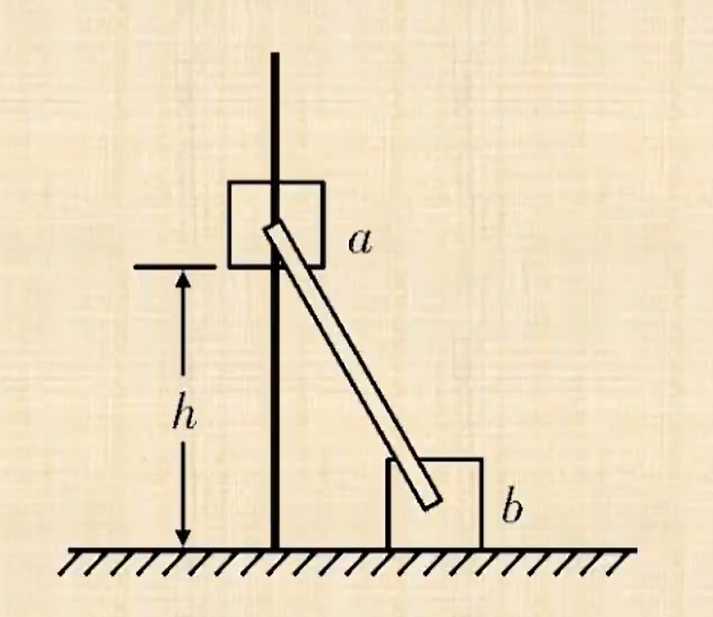
\includegraphics[width=0.34\linewidth]{image/45}
        \end{figure}
        \section{$C$平抛运动}
        \subsection{$C_1$平抛运动的基本原理}
        \subsubsection{$C_11$平抛运动的基本原理}
        一个图
        \vspace{2cm}
        
        两个关系
        \vspace{2cm}
        
        八个方程
        
       $v_x=v_0\,\,x=v_0t$
        
        $v_y=gt\,\,y=\frac{1}{2}gt^2$
       
        $v=\sqrt{{v_0}^2+{v_y}^2}\,\, \tan \alpha =\frac{v_y}{v_x}=\frac{gt}{v_0}$
        
        $s=\sqrt{x^2+y^2}\,\, \tan \beta =\frac{y}{x}=\frac{1}{2}\frac{gt^2}{v_0t}=\frac{1}{2}\tan \alpha $
        \subsubsection{$C_{12}$平抛运动的两个基本推论}
        
        速偏正切等于位偏正切的两倍$(\alpha\neq2\beta)$
        
        \text{末速度}v\text{的反向延长线过水平位移的中点}
        \subsubsection{$C_{13}$台阶问题}
        平抛遇到障碍物$\rightarrow$台阶问题$\rightarrow$找特殊点
        \vspace{3cm}
        \subsection{$C_2$平抛运动和斜面综合问题}
        \subsubsection{$C_{21}$顶抛底落型}
       \begin{figure}[H]
       	\centering
       	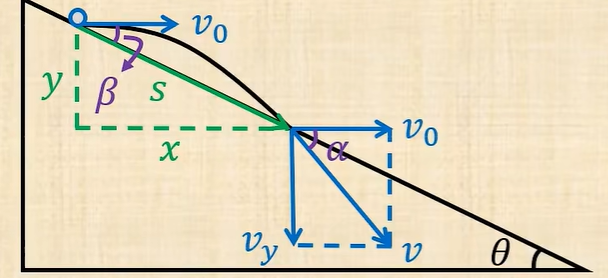
\includegraphics[width=0.3\linewidth]{image/47}
       \end{figure}
       
       已知$v_0$和$\theta$,求$t=\frac{2v_{0}\tan\theta}{g}$
        
       知二求其它:见八个方程
       
        距离斜面的最大高度H
        
        \subsubsection{$C_{22}$空抛垂落型}
        \begin{figure}[H]
        	\centering
        	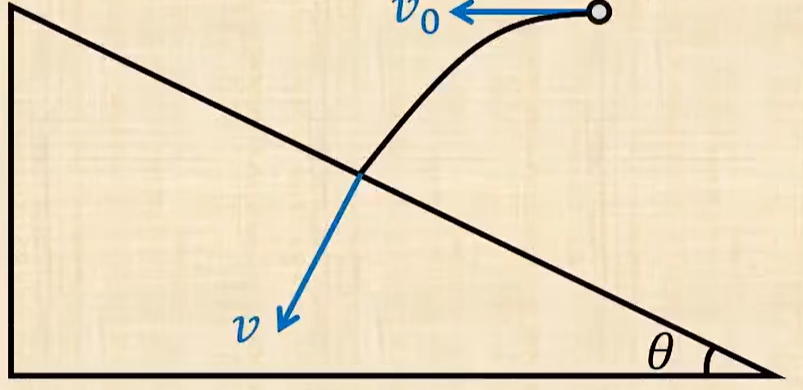
\includegraphics[width=0.3\linewidth]{image/48}
        \end{figure}
        
         已知$v_0$和$\theta$,求$t=\frac{v_{0}}{g\tan\theta}$
         
         知二求其它:见八个方程
         
         \subsubsection{$C_{23}$平抛撞圆}
         \begin{figure}[H]
         	\centering
         	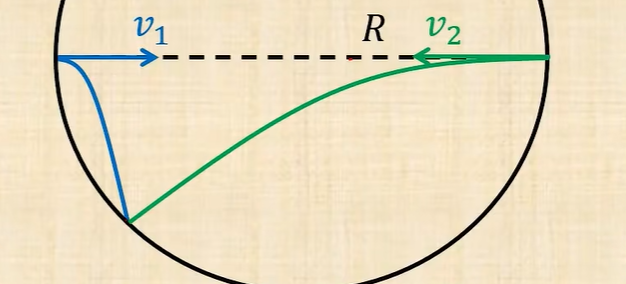
\includegraphics[width=0.3\linewidth]{image/49}
         \end{figure}
         
         \vspace{3cm}
         为什么沿着半径入射没法垂直撞击圆环?
         \section{$D$抛体运动}
         $\text{广义的抛体运动:受到恒力作用下的运动}\begin{cases}\text{直线:落体、竖直上抛、竖直下抛}\\\text{曲线:斜上抛、斜下抛、复杂抛体}&\end{cases}$
         \subsection{$D_1$斜上抛运动}
         
         \vspace{2cm}
         
         运动形式:
         
         最高点:
         
         对称性:上下等时间,同高等速
         
         \subsection{$D_2$抛体运动逆向思维}
         斜上抛运动在最高点两侧对称
         
         单独研究下降过程可视为平抛运动
         
        利用逆向思维单独研究上升过程也可视为平抛运动
        
        \section{$E$参考系变换(了解即可)}
        换参法则
        
        $\textcircled{1}$题型场景:二维传送带、直线上或空间内追及相遇
        
        $\textcircled{2}$换参法则:以谁为参考系就减去谁(的速度$v$和加速度$a)$
        
        $\textcircled{3}$矢量减法:先反向、再相加
        
        \section{$F$圆周运动}
        \subsection{$F_1$圆周运动基本原理}
        \subsubsection{$F_{11}$圆周运动基本公式}
        
        \vspace{3cm}
        
        \subsubsection{$F_{12}$拓展公式}
        $\text{转速}n=\begin{cases}
        	\text{单位:转}/s\,\,\rightarrow \omega =2\pi n\\
        	\text{单位:转}/\min \rightarrow \omega =\frac{2\pi n}{60}\\
        \end{cases}$
        
        \subsection{$F_2$同步转动}
        同心不一定同步,同步必有$\omega$相同
        
        同轴不一定同步,同步必有$\omega$相同
        
        同带不一定同步,同步必有$\upsilon$相同
        
        同齿不一定同步,同步必有$\upsilon$相同
        
        \subsection{$F_3$车轮的转动}
        \subsubsection{$F_{31}$受力情况}
        
        前轮:滚动摩檫力
        
        后轮(动力轮):静摩檫力
        
         \subsubsection{$F_{32}$运动形式}
         
         圆周运动+直线运动=摆线
         
         \subsection{$F_4$离心、向心、圆周}
         $ \text{圆运动的两种分类}\begin{cases}
         	\overset{}{\overset{\overset{}{\text{由}F_和\text{与}v\text{的方向共同决定}\begin{cases}
         					\text{夹角为锐角}\rightarrow \text{加速}\\
         					\text{夹角为直角}\rightarrow \text{匀速}\\
         					\text{夹角为钝角}\rightarrow \text{减速}\\
         		\end{cases}}}{\text{速率是否变化?}}\begin{cases}
         			\text{变速运动}\\
         			\text{匀速运动}\\
         	\end{cases}}\\
         	\mathop {\underset{\text{由供(}\mathbb{F} _{\text{合}}\text{法向分量)需(m}\frac{v^2}{r})\text{关系决定}}{\text{半径是否变化?}}\begin{cases}
         			\text{供}>\text{需}\rightarrow \text{近心运动}\\
         			\text{供}<\text{需}\rightarrow \text{离心运动}\\
         			\text{供}=\text{需}\rightarrow \text{圆周运动}\\
         	\end{cases}} \limits_{}\\
         \end{cases}$
         \subsection{$F_5$水平面内的匀速圆周运动}
         \subsubsection{$F_{51}$所有匀速圆周的底层原理}
         所有匀速圆周的底层原理:反向添加$ma$当成惯性力,然后写平衡方程
        \vspace{6cm}
        
         \subsubsection{$F_{52}$匀速圆周的临界状态}
         
         \vspace{3cm}
         
         \subsubsection{$F_{53}$同盘转动}
         \begin{figure}[H]
         	\centering
         	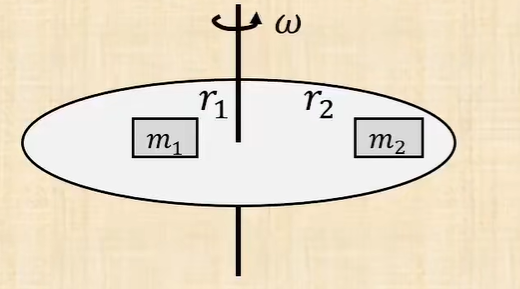
\includegraphics[width=0.3\linewidth]{image/51}
         \end{figure}
         
         滑动看内外:$r\text{越大,}\omega_0\text{越小,越容易被甩出}$
         
         系统看质心
         
         \vspace{2cm}
         
         剪断比临界
         
         \begin{example}
         $	\text{若}m_1=m_2=1\text{kg,}r_2=2r_1=2\text{m,当系统开始}\text{滑动的瞬间,剪断细线,则}m_1\text{和}m_2\text{会如何运动}?$
         \end{example}
         
         \vspace{3cm}
         
         内力看拔河:圆周惯性,先外后内;摩擦不够,拉力来凑
         \begin{example}
         	$\text{若}m_1=m_2=1\text{kg,}r_2=2r_1=2\text{m},\mu=0.1,\text{ 当转轴角速度等于系统开始滑动临界角}\text{速度的}\\\frac{\sqrt{2}}2\text{倍时,求细线上的拉力}T\text{和两个物体受到}\text{的静摩擦力。}$
         \end{example}
         \vspace{2cm}
         
         \chapter{天体运动}
	         \section{$A$万有引力定律}
	         \subsection{$A_1$万有引力公式}
	         定律公式:$F_{\text{万}}=\text{G}\frac{m_1m_2}{r^2}$
	         
	        $\text{条件:两个球体间的引力、两个距离很远的任意形状物体间的引力}$ 
	        
	        参数:
	        
	        $F_{\text{万}}:\text{引力的大小。注意这是标量式}$
	        
	        $m_1m_2:$两个球体的质量积
	        
	        $r:$天体球心距
	        
	        
	        G: 万有引力常量G$=6.67\times10^{-11}$N·m$^2/\mathrm{kg}^2$,卡文迪什扭秤实验测出
	        (也叫卡文迪许)
	        
	        \subsection{$A_2$非球体万有引力计算}
	        
	        方法:对称填补法
	        \vspace{3cm}
	        
	        \section{$B$环绕模型}
	        \subsection{$B_1$条件与暗示}
	        
	        圆周/匀速圆周/圆轨道
	        
	        \subsection{$B_2$解题公式组}
	        $ (r\text{球心距)G}\frac{Mm}{r^2}=m\frac{v^2}r=m\omega^2r=m\frac{4\pi^2}{T^2}r=ma$
	        \subsection{$B_3$公转五参数}
	       $ v=\sqrt{\frac{\mathrm{G}M}{r}}\left(v,M,r\right) \omega=\sqrt{\frac{\mathrm{G}M}{r^{3}}} \left(\omega,M,r\right) T=\sqrt{\frac{4\pi^{2}r^{3}}{\mathrm{G}M}}\left(T,M,r\right) a=\frac{\mathrm{G}M}{r^{2}}\left(a,M,r\right)$
	       \subsection{$ B_4$同心不同轨}
	       $\text{同心不同轨}\left\{ \begin{array}{l}
	       	\text{同一中心天体时}:\text{高轨低速大周期}\\
	       	\text{同一中心天体且绕行天体质量}m\text{相同:大机大势大能量}\\
	       \end{array} \right. $
	       \subsection{$B_5$近地卫星}
	       $\text{近地卫星}\begin{cases}\text{普通卫星}:r=R+h\\\text{近地卫星}\cdot h=0\text{时}\quad r=R\end{cases}$
	       \section{$C$黄金代换}
	       \subsection{$C_1$重力和万有引力的关系}
	       \vspace{3cm}
	       
	       \subsection{$C_2$黄金代换的三个公式和两个比例}
	       \subsubsection{$C_{21}$地内式}
	       
	       \vspace{1cm}
	       
	       \subsubsection{$C_{22}$地表式}
	       
	       \vspace{1cm}
	       
	       \subsubsection{$C_{23}$地外式}
	       
	       \vspace{1cm}
	       
	       \section{$D$质量密度计算}
	       \subsection{$D_1$中心天体质量计算}
	       \subsubsection{$D_{11}$选择题易错点}
	       
	       绕行天体质量不可求!
	       
	       \subsubsection{$D_{12}$知己}
	       知己:(知道中心天体参数求中心天体质量M)——借助$g_{\text{外}}$和$g_{\text{表}}$两类黄金代换
	       
	       \subsubsection{$D_{13}$知彼}
	       知彼:(知道绕行天体参数求中心天体质量M)$\{v\quad\omega/T \quad r\quad a\}$任意知二→求M
	       \vspace{2cm}
	       
	       \subsection{$D_2$中心天体密度计算}
	        \subsubsection{$D_{21}$选择题易错点}
	       
	       绕行天体密度不可求!
	       
	       \subsubsection{$D_{22}$知己}
	       知己:(知道中心天体参数求中心天体质量$\rho$)——借助$g_{\text{外}}$和$g_{\text{表}}$两类黄金代换
	       
	       \subsubsection{$D_{13}$知彼}
	       知彼:(知道绕行天体参数T求中心天体质量$\rho$)$\rho=\frac{3\pi}{GT^2}$
	       \vspace{2cm}
	       
	       T的三层含义:
	       
	       $\text{近地卫星周期}$
	       
	       $\text{ 甩出周期(赤道地表物体}\underline{\text{恰好被甩出时中心天体自转周期}})$
	       
	       $ \text{分解周期(中心天体}\underline{\text{恰好分解时中心天体自转周期)}}$
	       \section{$E$开普勒三大定律}
	       \subsection{$E_1$开普勒第一定律}
	       $\text{太阳系所有行星轨道都是椭圆,太阳位于椭圆的一个焦点上}$
	       
	       \subsection{$E_2$开普勒第二定律}
	       $\text{同一轨道的开二表述}:\text{同一轨道、相同时间},\text{连线扫过的面积相等}$
	       
	       $\text{不同轨道的开二表述}:\text{不同轨道、相同时间},(\text{大)轨道扫过面积更大}$
	       
	       $\text{两点速度的开二推论}:\text{远近点}:\frac{v_1}{v_2}=\frac{r_2}{r_1}; \text{其他点}:\frac{v_3}{v_4}\approx \frac{r_3}{r_4};$
	       
	       \subsection{$E_3$开普勒第三定律}
	       $ \frac{r^3}{T^2}&&=k\begin{cases}
	       	r:\text{椭圆半长轴或圆半径}\\
	       	k:\text{只和中心天体质量}M\text{有关}\\
	       	T:\text{比较正圆和椭圆的周期}\\
	       \end{cases}&&$$&&\mathrm{G}\frac{Mm}{r^2}&&=m\frac{4\pi ^2}{T^2}r\rightarrow \frac{GM}{4\pi ^2}&&=\frac{r^3}{T^2}
	       $
	       
	       \section{$F$三大宇宙速度}
	       \subsection{$F_1$第一宇宙速度}
	       (相对于行星而言)最小发射速度、最大环绕速度、环绕速度、近地卫星线速度
	       
	       计算:
	       
	       \subsection{$F_2$第二宇宙速度}
	       相对于行星来说:逃逸速度
	       \subsection{$F_3$第三宇宙速度}
	       相对于恒星来说:脱离速度
	       \section{$G$同步卫星}
	       \subsection{$G_1$同步卫星的定义}
	       
	       1.和中心天体自转周期相同
	       
	       2.赤道卫星
	       
	       3.顺行轨道
	       
	       \begin{remark}
	       	\text{已知地球自转周期}$T_\text{自转}$,十有八九都是暗示$T_\text{同步}$
	       \end{remark}
	       \subsection{$G_2$同步卫星参数比较}
	       \subsubsection{$G_{21}$同一中心天体的多个同步卫星}
	       
	       \vspace{3cm}
	       
	       \subsubsection{$G_{22}$同一中心天体的同步卫星和非同步卫星比较}
	       高轨低速大周期、大机大势大能量
	       
	       \subsection{$G_3$卫星与地表物体进行比较}
	        \subsubsection{$G_{31}$同步卫星比静止物体}
	        方法:回归同步转动
	       \begin{figure}[H]
	       	\centering
	       	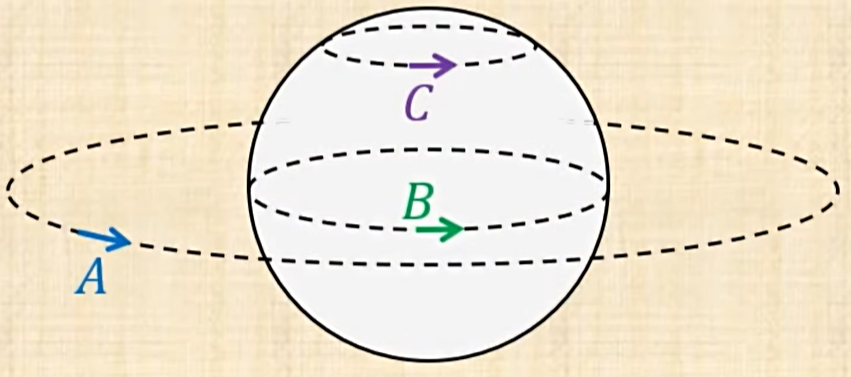
\includegraphics[width=0.3\linewidth]{image/52}
	       \end{figure}
	       \vspace{3cm}
	       
	       \subsubsection{$G_{32}$非同步卫星比静止物体}
	       方法:\text{用同卫做天地的桥梁}
	       \vspace{3cm}
	       
	       \subsection{$G_4$常见的天体与卫星常识}
	       
	       地球半径$R_\text{地}\approx6400km$
	       
	       地球公转周期:1年
	       
	       地球自转周期:1天
	       
	       地球近地卫星周期:84分钟
	       
	       月球半径$R_\text{月}\approx1700$ km
	       
	       月球表面重力加速度$g_\text{月}\approx1.63$ m/s$^2\approx\frac16g_\text{地}$
	       
	       月球公转周期:1个月
	       
	       \section{H变轨模型和对接问题}
	       \subsection{$H_1$如何变轨}
	       $\text{正圆轨}\longleftrightarrow\text{椭圆轨}\begin{cases}\text{切点处变轨}\\\text{小轨变大轨:切点加速}\\\text{大轨变小轨:切点减速}\end{cases}$
	       
	       $\text{正圆轨}\longleftrightarrow\text{正圆轨}\begin{cases}\text{不存在切点}\\\\\text{做辅助椭圆轨道}\\\\\text{经切点两次变轨}&\end{cases}$
	       
	       \section{$H_2$如何比较切点速度}
	       \begin{figure}[H]
	       	\centering
	       	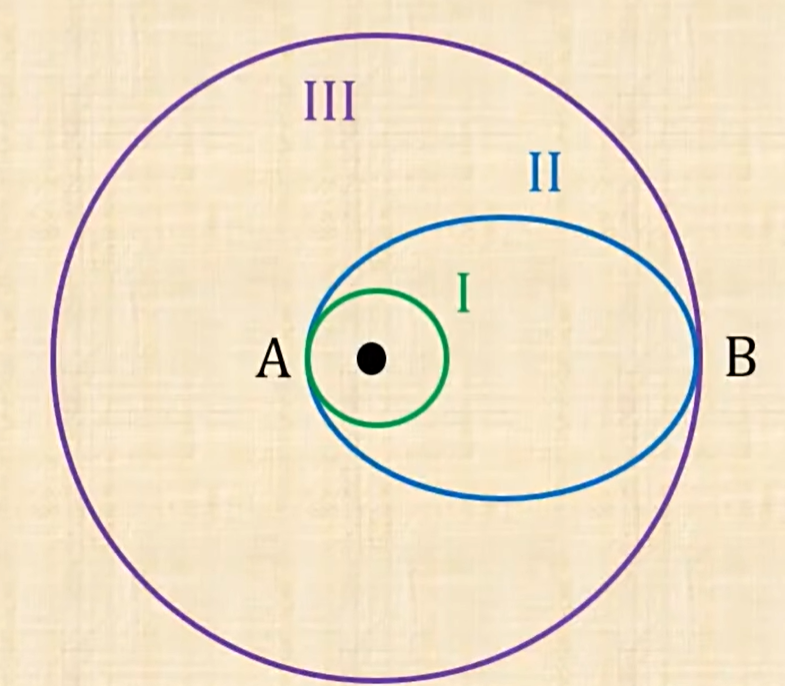
\includegraphics[width=0.3\linewidth]{image/53}
	       \end{figure}
	       
	       \section{$H_3$如何比较正圆轨道能量}
	       \begin{figure}[H]
	       	\centering
	       	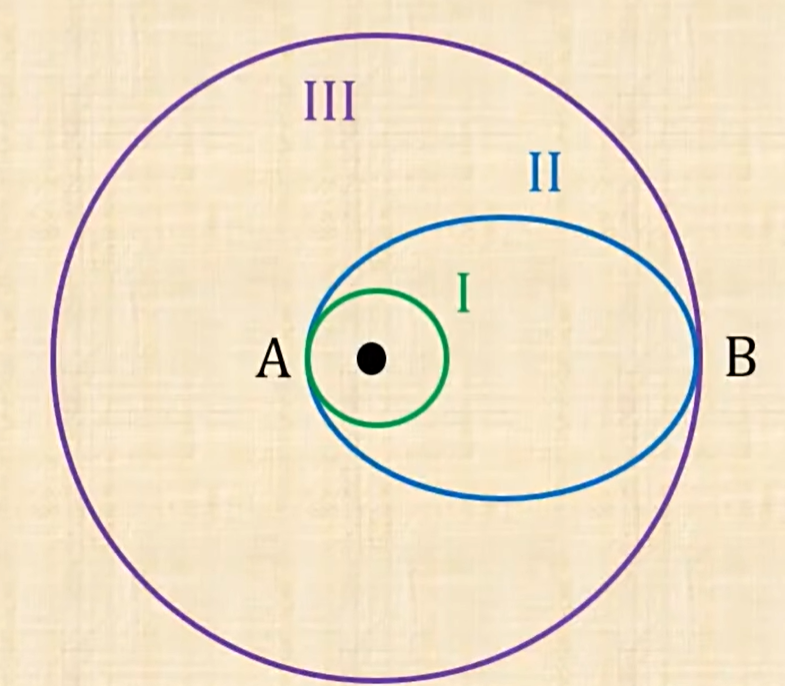
\includegraphics[width=0.3\linewidth]{image/54}
	       \end{figure}
	       
	       \section{$H_4$如何比较切点加速度}
	       \begin{figure}[H]
	       	\centering
	       	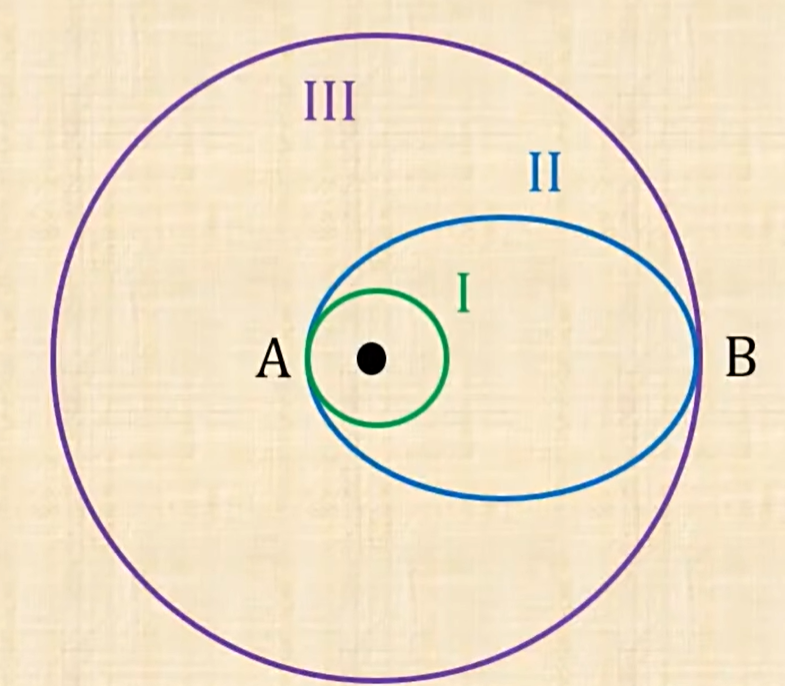
\includegraphics[width=0.3\linewidth]{image/54}
	       \end{figure}
	       
	       \section{$H_5$如何比较椭圆轨}
	       \begin{figure}[H]
	       	\centering
	       	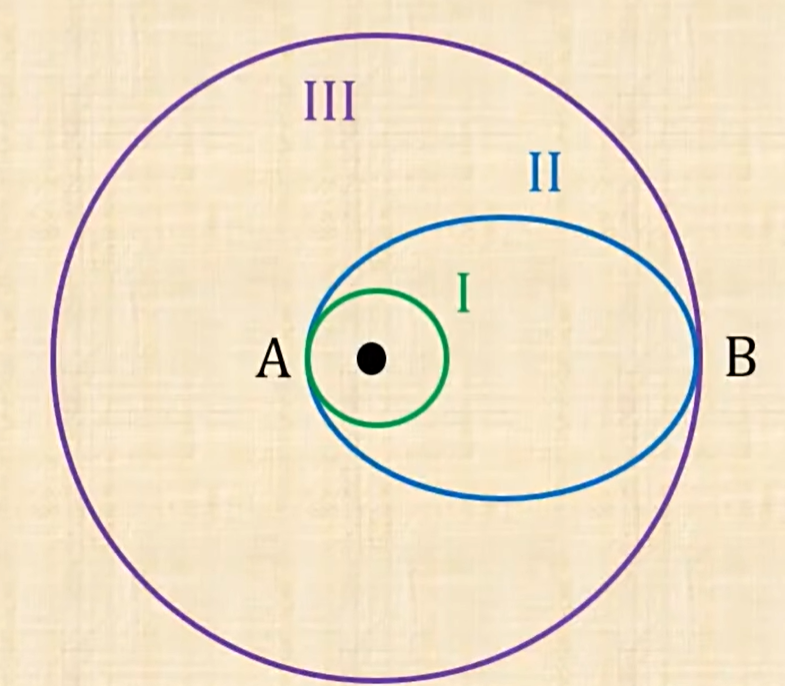
\includegraphics[width=0.3\linewidth]{image/54}
	       \end{figure}
	       \section{$I$多星问题}
	       \subsection{$I_1$双星问题}
	       \subsubsection{$I_{11}$参数比较}
	       四同——四个参数相同
	       \vspace{2cm}
	       
	       三反——三个参数的比等于质量的反比
	       \vspace{2cm}
	       \subsubsection{$I_{12}$重点计算 }
	        $\{\text{球心距}L,\text{总质量}M_\text{总}{\text{、周期}T}\}\text{ 知二求一}$
	        \vspace{2cm}
	        
	        \subsection{$I_2$多星问题}
	        \subsubsection{$I_{21}$多星问题一般处理方法}
	        \vspace{3cm}
	        
	        \subsubsection{$I_{21}$系统质心求解方法}
	        \vspace{3cm}
	        
	        \subsection{$I_3$拉格朗日点}
	        \subsubsection{$I_{31}$什么是拉格朗日点?}
	        \begin{figure}[H]
	        	\centering
	        	\includegraphics[width=0.3\linewidth]{image/55}
	        \end{figure}
	        
	        $\textcircled{1}$系统:双星系统中引入一个质量极小的第三颗星
	        
	        $\textcircled{2}$特征:第三星相对双星静止(共同$T$、稳定$r$)
	        
	        $\textcircled{3}$数量:共五个,其中$L_4$、$L_5$常在竞赛中考查
	        
	        \subsubsection{$I_{32}$题型总结}
	        
	         $\textcircled{1}$同步转动$:\text{周期T和角速度}\omega\text{相同的同轴转动}$
	         
	         $\textcircled{2}$:轨道计算
	         
	         \vspace{3cm}
	         
	         \begin{remark}
	         	
	         	$\begin{aligned}&1\text{若}M\gg m\text{,则}O\text{点近似位于}M\text{球心。}\\&2\text{否则:}r_M=r\frac m{M+m}\text{、}r_m=r\frac M{M+m}\end{aligned}$
	         \end{remark}
	         \section{$J$天体的追击相遇问题}
	         \subsection{$J_1$一种题型}
	         对象:绕同一中心天体公转的2个或多个天体
	         
	         题型:两绕行天体相距最近
	         
	         $\textcircled{1}$相遇 $\textcircled{2}$近点通信 $\textcircled{3}$行星冲日
	         
	          \subsection{$J_2$两种方法}
	          
	         $ \text{方法}\textcircled{1}\text{:常规参考系}+\text{角度关系}$
	         \vspace{2cm}
	         
	         $\text{方法}\textcircled{2}\text{:以慢为系}+\text{角度关系}$
	         
	         \subsection{$J_3$三个变形}
	         
	         $\text{变形}\textcircled{1}{:}\text{ 不同点出发 变形}\textcircled{2}{:}\text{ 反向绕行 变形}\textcircled{3}{:}\text{ 相距最远}$
	         \chapter{功与能}
	         \section{$A$功的公式}
	         \subsection{$A_1$恒力做功}
	         
	         $W=F\cdot s\cdot\cos\theta\text{ 力和位移夹角}\\\text{力的大小力作用点的位移大小}$
	         
	         做功条件:有力,有位移,角度不等于90
	         
	         $\text{共线力做功 }\begin{cases}Fs\text{同向:}W=+Fs\\Fs\text{反向:}W=-Fs\end{cases}$
	         
	         \begin{remark}
	         	功是标量,但是其比大小看绝对值
	         \end{remark}
	         
	          \subsection{$A_2$定力做功}
	          
	          方式一:平均力 一一对于随位移均匀变化的力
	          
	          方式二:求面积 一一$F-\underline{s}$图像的面积是做功
	          
	          方式三:动能定理
	          
	           \subsection{$A_3$变力做功}
	           
	           方法:动能定理,微元法
	           \section{$B$功能关系}
	           \subsection{$B_1$重力做功与重力势能}
	           功能关系:  \text{高度升高,重力做负功},\text{高度降低,重力做负功}
	           
	           \text{重力做功:和路径无关只和初末位置有关}
	           
	          $ \text{重力势能公式:}E_{\mathfrak{p}}=mgh\text{(距}0\text{势能面的高度)}$
	          
	          \subsection{$B_2$弹簧弹力做功与弹性势能}
	          
	          $\text{弹性势能定理:}W_{AB}=E_{\mathrm{p}A}-E_{\mathrm{p}B}$
	          
	          \text{弹簧弹力做正功,弹性势能减小},\text{弹簧弹力做负功,弹性势能增大}
	          
	          $\text{弹性势能公式:}E_{\mathfrak{p}}=\frac12k(\Delta x)^2$
	          
	         \begin{remark}
	         	万不得已不要用
	         \end{remark}
	         
	         
	         \subsection{$B_3$摩檫力做功与摩擦热能}
	         \subsubsection{$B_{31}$摩檫力功热公式}
	         $\begin{aligned}&\text{摩擦力功热公式}&\text{功: }W_f=f\cdot s\cdot(\cos\theta)&(s\text{为对地位移})\\&&\text{热: }Q_f=f\cdot\Delta s&(\Delta s\text{为相对位移,注意不是相对路程})\end{aligned}$
	         
	         \subsubsection{$B_{32}$斜面推论}
	         $\text{斜面上摩擦力做功=投影水平面摩擦力做功}$
	         
	         \vspace{2cm}
	          
	          \subsubsection{$B_{33}$摩檫力做功和产热关系}
	          \text{摩擦力负功数值}=\text{正功数值}+\text{摩擦产热}
	          \subsection{$B_4$运动过程中的能量转换}
	          \text{绝大部分的运动过程:人自己对自己做功}
	          
	          所有不知去向的能量:转化为内能
	          \subsection{$B_5$不能看成质点的物体的做功}
	          \text{对象:有质量的绳、有质量的流体}
	          
	          \text{套路:分段研究找重心(规则物体重心位于几何中心)}
	          \section{$C$功能关系}
	          \subsection{$C_1$过程问题}
	          过程问题:包括直线、曲线、圆周、平抛等等
	          
	          方法:过程写动能 $W_{\text{合}}=\frac{1}{2}mv_{\text{末}}^{2}-\frac{1}{2}mv_{\text{初}}^{2}$
	          
	         $ \begin{aligned}&\text{法一:求}F_\text{合,再求做功}\\&\text{法二:先求每个力的做功,再求和}\end{aligned}$
	         
	         \subsection{$C_2$状态写牛二}
		      \subsubsection{$C_{21} $弹簧的两组套路方程}
		      
		      题干信息1:做功$W_\text{弹、弹性势能}E_\mathrm{p}$、运动/做功过程(过程)
		      
		      题干信息2:劲度系数$k$(状态)
		      
		      \subsubsection{$C_{22} $轻绳的五个相等}
		      
		      同一条绳子拉力$T$相等
		      
		      绳两端沿绳方向位移x相等
		      
		      绳两端沿绳方向速度$\upsilon$相等
		      
		      绳两端沿绳方向加速度$a$相等
		      
		      绳两端力做功大小相等
		      \subsubsection{$C_{23} $轻杆的五个相等}
		      
		      $\begin{aligned}
		      	&\text{同一条活}\text{杆两端弹力T相等} \\
		      	&\text{活杆两端}\text{沿杆方向位移x相等} \\
		      	&\text{活杆两端}\text{沿杆方向速度v相等} \\
		      	&\text{活杆两端} \text{沿杆方向加速度a相等} \\
		      	&\text{活杆两端力做功大小相等(一正一负)} \\
		      \end{aligned}$
		      
		      \section{$D$能量守恒和机械能守恒}
		      \subsection{$D_1$能量守恒}
		      
		      条件:$\text{“系统/单体和外界没有能量交换}$
		      
		      方程:$ \begin{aligned}&\text{变量式:}\Delta E_\text{增}=\Delta E_\text{减}(\text{(多用于定量计算)}\\&\text{总量式:}E_1+E_2+\cdots+E_n=\text{定值}=E_1^{\prime}+E_2^{\prime}+\cdots+E_n^{\prime}\text{(多用于定性分析)}\end{aligned}$
		      
		      \subsection{$D_2$机械能守恒}
		      
		      $\begin{aligned}\text{对象为单体}\to\text{机械能定理(}\Delta E_\text{机}=W_{\text{其}}\\\text{对象为系统}\to\text{先写能量守恒}\end{aligned}$
		      
		      \subsection{$D_3$常见的机械能刚性损失}
		      \vspace{3cm}
		      
		      \subsection{$D_4$连续体能量转化问题}
		      
		      $\begin{aligned}&\text{处理方法:微元}\Delta t\text{、}\Delta V\text{、}\Delta m\text{;然后计算能量流动和转化}\\&\text{同类题型:连续体动量问题(冲力方程:}F=\rho Sv^2)\end{aligned}$
		     
		       \section{$E$机车启动}
		       \subsection{$E_1$恒定功率启动}
		       \subsubsection{$E_{11}$思维过程}
		       
		       $ P_0\text{不变}\to v\text{增大}\to F_\text{ 牵}{\text{减小}\to}a\text{减小(运动形式:}a\text{减小的加速运动)}$
		       
		       恒定功率$P_0$启动图像
		       
		       \vspace{3cm}
		       
		       \subsection{$E_2$恒定加速度启动}	       
		       \subsubsection{$E_{21}$思维过程}
		       $a\text{不变}\to v\text{增大}\to F_\text{态不变 }\to P\text{增大(当}P=P_0\text{后,相当于恒}P\text{启动})$
		       
		       \subsection{$E_3$变加速过程中的位移$s$和时间$t$}
		       
		       方法:动能定理
		       
		       \subsection{$E_4$突变问题}
		       \vspace{3cm}
		       
		       \section{$F$功能图像}
		       \subsection{$F_1$能量-位移图像}
		       \subsubsection{$F_{11}$动能-位移}
		       \vspace{1cm}
		       
		       \subsubsection{$F_{12}$机械能-位移}
		       \vspace{1cm}
		       
		       \subsubsection{$F_{12}$机械能-位移}
		       \vspace{1cm}
		       
		       \subsubsection{$F_{13}$重力势能-位移}
		       \vspace{1cm}
		       
		       \subsubsection{$F_{14}$摩擦产热-位移}
		       \vspace{1cm}
		       
		       
		       \subsection{$F_2$能量-其它图像}
		       
		       $\left. \begin{array}{r}
		       	\text{能量一能量图像}\\
		       	\text{能量}-\text{时间图像}\\
		       	\text{能量一速度图像}\\
		       \end{array} \right\} \text{解析式}\rightarrow \text{转化为一二次函数}$
		       
		       \vspace{3cm}
		       \subsection{$F_3$做功-位移图像}
		       \vspace{3cm}
		       
		       \section{$G$竖直面内的圆周运动}
		       \subsection{$G_1$球绳圆周运动}
		       \subsubsection{$G_{11}$绳子无功}
		       $\text{拉力}(T)\text{时刻垂直}\textcircled{v}\to W=0$
		       
		       \subsubsection{$G_{12}$上升到最高位置}
		       $\begin{aligned}&\text{小题直接写:}\quad v_\text{高}\geq\sqrt{gR}\\&\text{大题混步骤:“}mg=m\frac{v^2}R\overset{:}{\operatorname*{\to}}v_\text{高}\geq\sqrt{gR}\end{aligned}$
		       
		       \subsubsection{$G_{13}$上不去怎么办?}
		       
		       $\text{下半圆--------原路返回 上半圆——斜上抛运动}$
		       
		        \subsubsection{$G_{14}$上不去怎么办?}
		        
		        $\text{弹力只能指向圆心}$
		        
		        \subsubsection{$G_{15}$拉力差推论}
		        $\text{最高点最低点拉力差恒为6mg}$
		        
		         \subsection{$G_2$球杆圆周运动}
		        \subsubsection{$G_{21}$杆力无功}
		        $\text{拉力}(T)\text{时刻垂直}\textcircled{v}\to W=0$
		        
		        \subsubsection{$G_{22}$上升到最高位置}
		        $ v_\text{高}\geq 0$
		        
		        \subsubsection{$G_{23}$上不去怎么办?}
		        
		       任何位置---原路返回
		        
		        \subsubsection{$G_{24}$上不去怎么办?}
		        
		        $\text{弹力可指向圆心,也可背对圆心}$
		        
		        \subsubsection{$G_{25}$拉力差推论}
		        $\text{最高点最低点拉力差恒为6mg}$
		        
		        \subsection{$G_3$位置写牛二}
		        \vspace{3cm}
		        
		        \subsection{$G_4$竖直圆周的脱轨问题}
		        
		        $\text{脱离特性:脱离位置的临界状态为弹力等于}0$
\end{document}